\documentclass{sig-alternate}
%\documentclass[conference]{IEEEtran}
%\documentclass[conference,final]{IEEEtran}

%\usepackage[numbers, sort, compress]{natbib}
\usepackage{graphicx}
\usepackage{amsmath}
\usepackage{amssymb}
\usepackage{color}
\usepackage{ifpdf}
%\usepackage{mdwlist}

%\usepackage{dcolumn}
\usepackage{float}
\usepackage[utf8]{inputenc}
\usepackage{multirow}
\usepackage{rotating}
\usepackage{subfigure}



%\usepackage[numbers, sort, compress]{natbib}
%\usepackage{latex8}
%\usepackage{float}
%\usepackage{times}    
\usepackage{url}
\usepackage{booktabs}
\usepackage{listings}   
\usepackage{paralist}    
\usepackage{wrapfig}    
%\usepackage[footnotesize,it]{caption}
\usepackage{multirow}
\usepackage{ifpdf}
%\usepackage{srcltx}
%\usepackage{subfigure}
\usepackage{xspace}
\usepackage{keyval}  
\usepackage{color}
\usepackage{comment}

\definecolor{listinggray}{gray}{0.95}
\definecolor{darkgray}{gray}{0.7}
\definecolor{commentgreen}{rgb}{0, 0.4, 0}
\definecolor{darkblue}{rgb}{0, 0, 0.4}
\definecolor{middleblue}{rgb}{0, 0, 0.7}
\definecolor{darkred}{rgb}{0.4, 0, 0}
\definecolor{brown}{rgb}{0.5, 0.5, 0}

\usepackage[normalem]{ulem}
\makeatletter
\def\cyanuwave{\bgroup \markoverwith{\lower3.5\p@\hbox{\sixly \textcolor{cyan}{\char58}}}\ULon}
\def\reduwave{\bgroup \markoverwith{\lower3.5\p@\hbox{\sixly \textcolor{red}{\char58}}}\ULon}
\def\blueuwave{\bgroup \markoverwith{\lower3.5\p@\hbox{\sixly \textcolor{blue}{\char58}}}\ULon}
\font\sixly=lasy6 % does not re-load if already loaded, so no memory problem.
\makeatother

\newif\ifdraft
\drafttrue
\ifdraft
\usepackage{xcolor}
\newcommand{\onote}[1]{ {\textcolor{cyan} { (***Ole: #1) }}}
\newcommand{\terminology}[1]{ {\textcolor{red} {(Terminology used: \textbf{#1}) }}}
\newcommand{\owave}[1]{ {\cyanuwave{#1}}}
\newcommand{\jwave}[1]{ {\reduwave{#1}}}
\newcommand{\alwave}[1]{ {\blueuwave{#1}}}
\newcommand{\jhanote}[1]{ {\textcolor{red} { ***shantenu: #1 }}}
\newcommand{\alnote}[1]{ {\textcolor{green} { ***andreL: #1 }}}
\newcommand{\amnote}[1]{ {\textcolor{blue} { ***andreM: #1 }}}
\newcommand{\smnote}[1]{ {\textcolor{brown} { ***sharath: #1 }}}
\newcommand{\pmnote}[1]{ {\textcolor{brown} { ***Pradeep: #1 }}}
\newcommand{\msnote}[1]{ {\textcolor{cyan} { ***mark: #1 }}}
\newcommand{\mrnote}[1]{ {\textcolor{purple} { ***melissa: #1 }}}
\definecolor{orange}{rgb}{1,.5,0}
\newcommand{\aznote}[1]{ {\textcolor{orange} { ***ashley: #1 }}}
\definecolor{dandelion}{cmyk}{0,0.29,0.84,0}
\newcommand{\mtnote}[1]{ {\textcolor{dandelion} { ***matteo: #1 }}}
\newcommand{\note}[1]{ {\textcolor{magenta} { ***Note: #1 }}}
\else
\newcommand{\onote}[1]{}
\newcommand{\terminology}[1]{}
\newcommand{\owave}[1]{#1}
\newcommand{\jwave}[1]{#1}
\newcommand{\alnote}[1]{}
\newcommand{\amnote}[1]{}
\newcommand{\aznote}[1]{}
\newcommand{\athotanote}[1]{}
\newcommand{\smnote}[1]{}
\newcommand{\pmnote}[1]{}
\newcommand{\jhanote}[1]{}
\newcommand{\msnote}[1]{}
\newcommand{\mtnote}[1]{}
\newcommand{\note}[1]{}
\newcommand{\mrnote}[1]{}
\fi

\newcommand{\cloud}{cloud\xspace}
\newcommand{\clouds}{clouds\xspace}
\newcommand{\pilot}{Pilot\xspace}
\newcommand{\pilots}{Pilots\xspace}
\newcommand{\pilotjob}{Pilot-Job\xspace}
\newcommand{\pilotjobs}{Pilot-Jobs\xspace}
\newcommand{\pilotcompute}{Pilot-Compute\xspace}
\newcommand{\pilotcomputes}{Pilot-Computes\xspace}
\newcommand{\pilotdata}{Pilot-Data\xspace}
\newcommand{\pilotdataservice}{Pilot-Data Service\xspace}
\newcommand{\pilotcomputeservice}{Pilot-Compute Service\xspace}
\newcommand{\computedataservice}{Compute-Data Service\xspace}
\newcommand{\pilotmapreduce}{PilotMapReduce\xspace}
\newcommand{\mrmg}{MR-Manager\xspace}
\newcommand{\pstar}{P*\xspace}
\newcommand{\pd}{PD\xspace}
\newcommand{\pj}{PJ\xspace}
\newcommand{\pjs}{PJs\xspace}
\newcommand{\pds}{Pilot Data Service\xspace}
\newcommand{\computeunit}{Compute-Unit\xspace}
\newcommand{\computeunits}{Compute-Units\xspace}
\newcommand{\dataunit}{Data-Unit\xspace}
\newcommand{\dataunits}{Data-Units\xspace}
\newcommand{\du}{DU\xspace}
\newcommand{\dus}{DUs\xspace}
\newcommand{\cu}{CU\xspace}
\newcommand{\cus}{CUs\xspace}
\newcommand{\su}{SU\xspace}
\newcommand{\sus}{SUs\xspace}
\newcommand{\schedulableunit}{Schedulable Unit\xspace}
\newcommand{\schedulableunits}{Schedulable Units\xspace}
\newcommand{\cc}{c\&c\xspace}
\newcommand{\CC}{C\&C\xspace}
\newcommand{\up}{\vspace*{-1em}}
\newcommand{\upp}{\vspace*{-0.5em}}
\newcommand{\numrep}{8 }
\newcommand{\samplenum}{4 }
\newcommand{\tmax}{$T_{max}$ }
\newcommand{\tc}{$T_{C}$ }
\newcommand{\tcnsp}{$T_{C}$}
\newcommand{\bj}{BigJob\xspace}
\newcommand{\MW}{Master-Worker\xspace}
\newcommand{\panda}{PanDA\xspace}
\newcommand{\apples}{AppLeS\xspace}

\newcommand{\I}[1]{\textit{#1}\xspace}
\newcommand{\B}[1]{\textbf{#1}\xspace}
\newcommand{\T}[1]{\texttt{#1}\xspace}
\newcommand{\C}[1]{\textsc{#1}\xspace}

\lstdefinestyle{myListing}{
  frame=single,   
  backgroundcolor=\color{listinggray},  
  %float=t,
  language=C,       
  basicstyle=\ttfamily \footnotesize,
  breakautoindent=true,
  breaklines=true
  tabsize=2,
  captionpos=b,  
  aboveskip=0em,
  belowskip=-2em,
  %numbers=left, 
  %numberstyle=\tiny
}      

\lstdefinestyle{myPythonListing}{
  frame=single,   
  backgroundcolor=\color{listinggray},  
  %float=t,
  language=Python,       
  basicstyle=\ttfamily \footnotesize,
  breakautoindent=true,
  breaklines=true
  tabsize=2,
  captionpos=b,  
  %numbers=left, 
  %numberstyle=\tiny
}



%  \setlength{\parskip}{0.05ex} % 1ex plus 0.5ex minus 0.2ex}
%  \setlength{\parsep}{0pt}
%  %\setlength{\headsep}{0pt}
%  \setlength{\topskip}{0pt}
%  \setlength{\topmargin}{0pt}
%  %\setlength{\topsep}{0pt}
%  \setlength{\partopsep}{0pt}

% This is now the recommended way for checking for PDFLaTeX:


\ifpdf
\DeclareGraphicsExtensions{.pdf, .jpg, .tif}
\else
\DeclareGraphicsExtensions{.eps, .jpg, .ps}
\fi

\tolerance=1000
\hyphenpenalty=10

\usepackage{lscape}

\usepackage{listings}

\lstnewenvironment{code}[1][]%
{
\noindent
%\minipage{0.98 \linewidth}
\minipage{1.0 \linewidth}
\vspace{0.5\baselineskip}
\lstset{
    language=Python,
%    numbers=left,
%    numbersep=4pt,
    frame=single,
    captionpos=b,
    stringstyle=\ttfamily,
    basicstyle=\scriptsize\ttfamily,
    showstringspaces=false,#1}
}
{\endminipage}

\begin{document}
\conferenceinfo{HPDC'13}{2013, New York, USA}
% \conferenceinfo{ECMLS'11,} {June 8, 2011, San Jose, California, USA.}
% \CopyrightYear{2011}
% \crdata{978-1-4503-0702-4/11/06}
% \clubpenalty=10000
% \widowpenalty = 10000

\title{A Fresh Perspective on Pilot-Jobs}

% \alignauthor
% Ben Trovato\titlenote{Dr.~Trovato insisted his name be first.}\\
%        \affaddr{Institute for Clarity in Documentation}\\
%        \affaddr{1932 Wallamaloo Lane}\\
%        \affaddr{Wallamaloo, New Zealand}\\
%        \email{trovato@corporation.com}
% % 2nd. author
% \alignauthor
% G.K.M. Tobin\titlenote{The secretary disavows
% any knowledge of this author's actions.}\\
%        \affaddr{Institute for Clarity in Documentation}\\
%        \affaddr{P.O. Box 1212}\\
%        \affaddr{Dublin, Ohio 43017-6221}\\
%        \email{webmaster@marysville-ohio.com}
% % 3rd. author
% \alignauthor Lars Th{\o}rv{\"a}ld\titlenote{This author is the
% one who did all the really hard work.}\\
%        \affaddr{The Th{\o}rv{\"a}ld Group}\\
%        \affaddr{1 Th{\o}rv{\"a}ld Circle}\\
%        \affaddr{Hekla, Iceland}\\
%        \email{larst@affiliation.org}
% \and  % use '\and' if you need 'another row' of author names
% % 4th. author
% \alignauthor Lawrence P. Leipuner\\
%        \affaddr{Brookhaven Laboratories}\\
%        \affaddr{Brookhaven National Lab}\\
%        \affaddr{P.O. Box 5000}\\
%        \email{lleipuner@researchlabs.org}
% % 5th. author
% \alignauthor Sean Fogarty\\
%        \affaddr{NASA Ames Research Center}\\
%        \affaddr{Moffett Field}\\
%        \affaddr{California 94035}\\
%        \email{fogartys@amesres.org}
% % 6th. author
% \alignauthor Charles Palmer\\
%        \affaddr{Palmer Research Laboratories}\\
%        \affaddr{8600 Datapoint Drive}\\
%        \affaddr{San Antonio, Texas 78229}\\
%        \email{cpalmer@prl.com}
% }

\date{}
\maketitle

\begin{abstract}
  There is no agreed upon definition of \pilotjobs; however a
  functional attribute of \pilotjobs that is generally agreed upon is
  they are tools/services that support multi-level and/or
  application-level scheduling by providing a scheduling overlay on
  top of the system-provided schedulers.  
  Nearly everything else is either specific to an
  implementation, open to interpretation or not agreed upon. For
  example, are \pilotjobs part of the application space, or part of
  the services provided by an infrastructure? We will see that
  close-formed answers to questions such as whether \pilotjobs are
  system-level or application-level capabilities are likely to be
  elusive. Hence, this paper does not make an attempt to provide
  close-formed answers, but aims to provide appropriate context,
  insight and analysis of a large number of \pilotjobs, and thereby
  bring about a hitherto missing consilience in the community's
  appreciation of \pilotjobs.  Specifically this paper aims to provide
  a comprehensive survey of \pilotjobs, or more generically of
  \pilotjob like capabilities.  A primary motivation for this work stems
  from our experience when looking for an interoperable, extensible
  and general-purpose \pilotjobs; in the process, we realized that
  such a capability did not exist. The situation was however even more
  unsatisfactory: in fact there was no agreed upon definition or
  conceptual framework of \pilotjobs.  To substantiate these points of
  view, we begin by sampling (as opposed to a comprehensive survey)
  ~\onote{a few lines above we say that we're doing a comprehensive
    survey!} some existing \pilotjobs and the different aspects of
  these \pilotjobs, such as the applications scenarios that they have
  been used and how they have been used. The limited but sufficient
  sampling highlights the variation, and also provides both a
  motivation and the basis for developing an implementation agnostic
  terminology and vocabulary to understand \pilotjobs; Section \S3
  attempts to survey the landscape/eco-system of \pilotjobs.  With an
  agreed common framework/vocabulary to discuss and describe
  \pilotjobs, we proceed to analyze the most commonly utilized
  \pilotjobs and in the process provide a comprehensive survey of
  \pilotjobs, insight into their implementations, the infrastructure
  that they work on, the applications and application execution modes
  they support, and a frank assessment of their strengths and
  limitations.  An inconvenient but important question -- both
  technically and from a sustainability perspective that must be
  asked: why are there so many similar seeming, but partial and
  slightly differing implementations of \pilotjobs, yet with very
  limited interoperability amongst them?  Examining the reasons for
  this state-of-affairs provides a simple yet illustrative case-study
  to understand the state of the art and science of tools, services
  and middleware development.  Beyond the motivation to understand the
  current landscape of \pilotjobs from both a technical and a
  historical perspective, we believe a survey of \pilotjobs is a
  useful and timely undertaking as it provides interesting insight
  into understanding issues of software sustainability.
  % believe that a survey of \pilotjobs provides and appreciation for
  % the richness of the \pilotjobs landscape.  is
  % not to discuss the \pstar conceptual framework, but That led to
  % the \pstar model.
\end{abstract}

\section{Introduction}\label{sec:intro}

\jhanote{Generally not good style to begin new subsection immediately
  after section starting}

The seamless uptake of distributed infrastructures by scientific
applications has been limited by the lack of pervasive and
simple-to-use abstractions at multiple levels – at the development,
deployment and execution stages. Of all the abstractions proposed to
support effective distributed resource utilization, a survey of actual
usage suggested that \pilotjobs were arguably one of the most
widely-used distributed computing abstractions – as measured by the
number and types of applications that use them, as well as the number
of production distributed cyberinfrastructures that support them.

\jhanote{Now develop the following paragraph along the lines of: Why
  have \pilotjobs been successful?}

The fundamental reason for the success of the \pilotjob abstraction is that
\pilotjobs liberate applications/users from the challenging requirement of
mapping specific tasks onto explicit heterogeneous and dynamic resource pools.
In other words, at least in part, due to the decoupling between task/workload
specification and task management. \pilotjobs also improve the efficiency of
task assignment and shield applications from having to load-balance tasks
across such resources.\onote{not sure if 'load-balance'  is appropriate here}
Another concern often addressed by \pilotjobs is fault
tolerance which commonly refers the ability of the \pilotjob system to verify
the execution environment before executing jobs. The \pilotjob abstraction is
also a promising route to address specific requirements of distributed
scientific applications, such as coupled-execution and application-level
scheduling~\cite{ko-efficient,DBLP:conf/hpdc/KimHMAJ10}.

%   \onote{I think the most important reasons why Pilot Jobs being so
%     popular (and re-invented over and over again) is that they allow
%     the execution of small (i.e., singe / few-core) tasks efficiently
%     on HPC infrastrucutre by massively reducing queueing time. HPC
%     sites (from schedulers to policies) have always been (and still
%     are) discrimatory against this type of workload in favor of the
%     large, tightly-coupled ones. Pilot-Jobs try to counteract. While
%     this is certainly not the main story that we want to tell, this
%     should IMHO still be mentioned. } \jhanote{This is definitely one
%     of the main reasons, but as Melissa pointed out it during RADICAL
%     call, it is by no means the only reason. Need to get the different
%     reasons down here.. then find a nice balance and description}

\jhanote{Although pilotjobs have solved/addressed many problems, now
    develop the problem with \pilotjobs themselves..}
A variety of PJ frameworks have emerged: Condor-G/
Glide-in~\cite{condor-g}, Swift~\cite{Wilde2011},
DIANE~\cite{Moscicki:908910}, DIRAC~\cite{1742-6596-219-6-062049},
PanDA~\cite{1742-6596-219-6-062041}, ToPoS~\cite{topos},
Nimrod/G~\cite{10.1109/HPC.2000.846563}, Falkon~\cite{1362680} and
MyCluster~\cite{1652061} to name a few. Although they are all, for the
most parts, functionally equivalent -- they support the decoupling of
workload submission from resource assignment -- it is often impossible
to use them interoperably or even just to compare them functionally or
qualitatively.  The situation is reminiscent of the proliferation of
functionally similar yet incompatible workflow systems, where in spite
of significant a posteriori effort on workflow system extensibility
and interoperability (thus providing post-facto justification of its
needs), these objectives remains difficult if not infeasible.

\section{A Preliminary Survey of Existing Pilot-Jobs
  Systems}\label{sec:prelim}


%\subsection{A Functional Approach to Pilot-Jobs}
%Many scientific communities began running into the same issues:

As distributed systems grew in capacity and capability, they also grew
in complexity and heterogeneity. For example, many machines
implemented their own batch queuing systems, and oftentimes these
systems varied from machine to machine.  The wide use of heterogenous
resources, resulted in the need for workload management across these
resources.  In order to harness the power of these heterogeneous
resources to run jobs, one particular solution proposed is that of
\pilotjobs

% , which have historically been used as a means of solving these
% issues.
% This gave rise to the the need for job submission management via batch
% queuing systems and middleware access also grew.
%We briefly discuss some specific uses of \pilotjobs below.

\pilotjobs are most commonly used for the execution of many tasks
through the use of a container job. They are often measured by
their throughput, that is, the number of tasks that they can complete
per second (tps), or alternatively, by the total number of tasks
executed. As such, \pilotjobs are used to achieve
high-throughput, for example, when using genome sequencing techniques
or ensemble-based applications. \pilotjobs have also been used for
parameter sweeps, chained tasks, and loosely-coupled but distinct
tasks. %note to self: cite these with papers

Multi-scale simulations have also benefited from the use of
\pilotjobs. A framework for load balancing via dynamic resource
allocation for coupled multi-physics (MPI-based) simulations using
\pilotjobs was demonstrated in Ref.~\cite{ko-efficient}.
This was achieved by dynamically assigning more processors to
jobs with longer runtimes, so that these jobs could accomplish their workload
in the same amount of wall-clock time as those with shorter runtimes.
This led to an overall reduction of jobs that were waiting to communicate
via MPI, and an overall reduction of the total simulation runtime.

\pilotjobs can be used for  simulations
 with varying numbers of tasks to complete, for example,
molecular dynamics simulations requiring task restart. These types of
 simulations may start with a fixed number of tasks but spawn
 more tasks in order to continue simulating. \pilotjobs can be
utilized for these types of dynamic simulations, because
new tasks can be fed to the \pilot at any time within a given
runtime. Without \pilotjobs, these simulations would have to
be resubmitted to the batch queue and wait for their time
to become active again~\cite{luckow2009adaptive}.

\pilotjobs have also been used to avoid queue wait times for many jobs
as well as harness and utilize different resources (with different
batch queueing systems) to do \textit{scale-across} simulations.
As a fault tolerant mechanism, many \pilotjob systems monitor
failed jobs and have the ability to restart them within the given
time frame of the \pilotjob's total runtime~\cite{1742-6596-219-6-062049,condor-g,nilsson2011atlas}.

\subsection{Landscape of \pilotjobs}\label{ssec:landscape}

\jhanote{I will write}

\subsection{Pilot-Job Systems Overview}
\label{ssec:informal}


% In order to appreciate \pilotjobs, we outline the evolution of
% \pilot-like capabilities ultimately leading to the creation of the
% first actual \pilotjob. We present a brief chronological order of
% \pilotjob-like systems, beginning with simple Master-Worker-based
% applications through advanced workload management systems.

% \subsubsection*{The Evolution of \pilotjobs}\label{sssec:evolution}

\jhanote{if we are calling this ``evolution'' we should be sure to
  discuss topics in chronological order. Melissa, can you please check
  that topics are in deed presented in chronological order and maybe
  even create a table of timelines. thanks}

\pilotjobs provide the ability to distribute workload across multiple systems and
offer an easy way to schedule many jobs at one time. This in turn improves the
utilization of resources, reduces the net wait time of a collection of tasks, and
also prevents saturation of resource batch queuing systems from high-throughput
simulations where many jobs need to be run at one time. While early \pilot-systems
solely provided this placeholder job mechanism, many of these system evolved to
more complex workload management systems. As applications began to utilize
distributed cyberinfrastructure, the workloads grew from small sets of short
running jobs to many jobs with either short or potentially long runtimes. There was
a need for more complex management of these workloads and additional capabilities
for user-level control of the tasks that would be executed within the placeholder
job. This drove the creation of the modern idea of \pilots.

\mrnote{Maybe we should change the figure? -- I am changing the 
overall text of this section but i have no idea how to make figures}

\pilotjob systems differ in their focus and architecture. Our preliminary
survey of existing \pilotjobs helped to identify three major layers that
these systems exhibit: (i) core \pilotjob functionality - this provides the 
minimally complete set of capabilities for a simple \pilotjob, (ii) advanced
\pilotjob functionality - a system that offers all of (i) plus a more sophisticated
resource management mechanism, and (iii) higher-level \pilot-based frameworks
- frameworks utilize \pilots for a specific use case, e.\,g.\ workflows or data analytics. 
As one can intuit from the above descriptions, existing \pilotjob systems maybe
overlap and overflow into these different layers, and each layer builds upon the
previous one. Therefore, we use these classification layers only as a means
to explain the basic progression of a \pilotjob system from simple scheduling
reservation mechanisms to more complete job management systems. A 
more semantically-rich terminology and classification scheme will be presented
in Sections \ref{sec:vocab} and \ref{sec:4}.


%Figure~\ref{fig:figures_classification} categorized \pilotjob systems into three
%layers: (i) core \pilotjob systems that solely provide a simple \pilot capability,
%(ii) advanced \pilotjob systems that offer sophisticated resource management
%capabilities based on \pilots, and (iii) higher level \pilot-based frameworks
%that utilize \pilots for a specific use case, e.\,g.\ workflows or data analytics.
%One of the important aspects of these layers is that they often overlap or
%have evolved from one another. Therefore, it is hard to classify 

\begin{figure}[t]
	\centering
		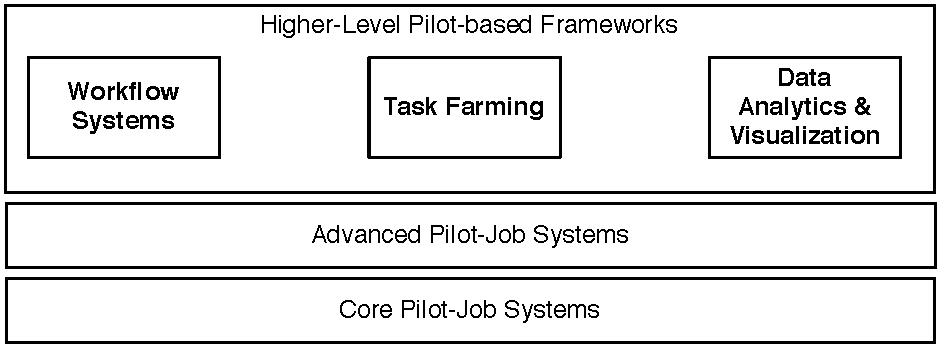
\includegraphics[width=0.45\textwidth]{figures/classification}
	\caption{Pilot-Job Classification: Different PJ systems focus
          on different parts of the distributed computing stack: (i)
          PJ systems that solely provide the \pilot capability, (ii)
          systems that offer resource management capabilities based on
          \pilots and (iii) applications, tools and services that
          utilize \pilots for resource management. \jhanote{we should
            make the three levels of the diagram consistent with the
            three categories, ``core PJ'' , ``advanced PJ'' and
            ``higher-level PJs'' . Also earlier comment about adding
            ``higher-level pilot-based frameworks'' to ``higher-level
            frameworks that can use pilot-jobs''.}}  \alnote{mention
          that these layers are not cleanly separated, add
          capabilities (outside)/properties (internal) of
          each layer, what is the overlap between the layers (how they
          interrelated?, what is the overlap?)?}
	\label{fig:figures_classification}
\end{figure}

In this section, we give a brief overview of different \pilotjob systems. As
grid computing advanced in its size and capabilities, the need for
job scheduling and time-sharing became more prevalent. Batch
queuing systems were installed to solve this problem, wherein a login
node accepted all job submissions and then the queuing system
divvied up the work to the worker nodes. 
The requirements of distributed applications, such as efficient load
balancing and resource utilization across multiple resources, drove
the need for user-level control of tasks and ease of use of job
descriptions for data driven
applications~\cite{ko-efficient}~\cite{DBLP:conf/hpdc/KimHMAJ10}, but
the concept of a \pilot was not the first type of application-level scheduling 
introduced.


After a 
discussion of pre-pilot systems in section~\ref{sec:prepilot}, we will discuss 
the three types of \pilotjob systems in-depth in sections~\ref{sec:corepj} -- 
\ref{sec:pjframeworks}.

\msnote{Im still uncomfortable with this classification. It feels awkward. And
on a more formal note, its weird that we classify at this stage, while only later in
the paper we start to define what "Core" functionality is.}
\mrnote{Yeah, I will take this into consideration}

\subsubsection{Pre Pilot-Job Systems}
\label{sec:prepilot}
\alnote{maybe merge with core pilotjobs}
\msnote{I agree with AL, as even "core" pilotjobs were/are not called pilots in
(their first incarnations).}

\pilotjobs have been used even before they
were named as such; we refer to these as pre-\pilotjob systems, a
prominent example of which is the Master-Worker (M-W) scheme and
associated frameworks.  In the context of distributed systems, the M-W
scheme was initially used of farming tasks from a master to a various
number of workers, and could easily be adapted to run in a
platform-independent way across the potentially heterogeneous
resources~\cite{masterworker, Goux00anenabling}. Master-Worker based
frameworks could respond to the dynamically changing resources by
adapting the number of workers to match the resource availability.

%Although Master-Worker schemes were important, they
%required application modification. \jhanote{last statement is unclear}
%\onote{I don't think that I agree with this
%statement. There are lots of independent master-worker frameworks, libraries
%and tools out there. What does 'application modification' mean here?}

BOINC is a volunteer-based, distributed master-worker framework that
also pre-dated \pilotjob
systems~\cite{Anderson:2004:BSP:1032646.1033223}. BOINC plays a
significant role in distributed computing in that it utilizes unused
computer cycles on the client-side in order to execute tasks given
from the server-side. Applications can be built on top of BOINC for
their own scientific endeavors; it was originally built for the
SETI@Home project, which uses Internet-connected computers to download
and analyze radio telescope data. Most often, these computers are
based around the world -- users merely have to download the client
program, and it runs in the background on their computer. The data is
then aggregated back on the server-side and analyzed. The idea of
farming out tasks in a distributed environment including personal
computers was powerful in that it essentially made a grid out of many
less powerful machines.

As the resources in the grid adopted more and more batch queuing
systems, users were forced to submit their jobs individually to a
scheduler. Oftentimes, the type of scheduler on a certain machine was
different than that of another machine. There was a need for managing
the heterogenous, dynamic grid environments, especially in terms of
dynamic scheduling. This drove the creation of
AppLeS~\cite{Berman:2003:ACG:766629.766632}, a framework for
application-level scheduling. For this purpose, AppLeS provides an
agent that can be embedded into an application enabling the
application to acquire resources (e.\,g.\ via Globus, SSH or Legion)
and efficiently schedule tasks onto these. Further, AppLeS provides
different application templates, e.\,g.\ for parameter sweep,
master-worker and moldable parallel applications.

The rise of application-level scheduling, as in AppLeS, opened new
possibilities to Grid environments. The concept of application-level
scheduling was extended to include long-term performance prediction in
heterogenous Grid environments via the Grid Harvest Service (GHS)
system~\cite{ghs}. GHS provides a prediction model that was derived by
probability analysis and simulation and useful for large-scale
applications in shared environments. Its prediction models and task
scheduling algorithms are utilized in the placement of tasks across
Grid resources. GHS supports three classes of task scheduling: (i)
single task, (ii) parallel processing, and (iii) meta-task. The
performance evaluation and modeling in conjunction with task-specific
management (such as placement, scheduling, and execution) allows the
utilization of many heterogenous resources in an efficient manner.

Although pre-pilot systems, such as AppLeS, gave user-level control of
scheduling, queue reservation time still was an issue. This brought
about the idea of placeholder
scheduling~\cite{Pinchak02practicalheterogeneous,
  Singh:2008:WTC:1341811.1341822}. A placeholder was an early \pilot
mechanism in that it was an abstraction layer above the various batch
queuing systems available on different resources. It held a
\textit{place} in the regular batch queue, and when it became active,
it could pull tasks to execute.  Placeholder scheduling was
advantageous in that it did not require any special superuser
privileges on the machines, which was something most grid users did
not have access to. It also provided a means of load balancing across
the different resources. As placeholder scheduling evolved, it came to
include dynamic monitoring and throttling of the different
placeholders based on the queue times on the machines.


\subsubsection{Core Pilot-Job Systems}
\label{sec:corepj}
\alnote{add BigJob}

\jhanote{I think the very brief description of the various examples of
  the three types is helpful, but the individual subsubsections need
  to go on beyond simply describing the examples. The subsubsections
  open out well with some description but they need to close out after
  they distill what is common to the grouped examples, so as to
  understand better the distinction between categories}

Core \pilotjob systems focus on the basic \pilot capabilities, i.\,e.\ the
provisioning of the placeholder job capability. 
% Various Master-Worker systems
% that provide such a mechanism (e.\,g.\ Nimrod-G~\cite{10.1109/HPC.2000.846563}). 
Condor-G/Glide-In is the most well-known \pilotjob system. Further examples for
lightweight \pilotjob systems are: ToPos~\cite{topos},
MyCluster~\cite{Walker:2007:PAC:1285840.1285848},
GridBot~\cite{Silberstein:2009:GEB:1654059.1654071} and LGI~\cite{lgi}.


Nimrod-G~\cite{10.1109/HPC.2000.846563}, DIANE~\cite{diane-thesis} and Work
Queue~\cite{workqueue-pyhpc2011} are examples of Master-Worker systems that
utilize a placeholder agent that dispatches and manages tasks. For example,
Nimrod-G utilizes a Job Wrapper that is responsible for pulling a task and its
associated data and then manages the execution of this task. While modern
\pilotjobs often acquire resources opportunistically and then distribute tasks
to resources they were able to acquire, Nimrod-G utilizes a central,
cost-based scheduler.

Condor-G/Glide-in~\cite{condor-g} is one of the pioneers of the \pilotjob
concept. Glide-in is a mechanism by which user can add remote grid resources
to the local condor pool and run their jobs on the added resource the same way
that all condor jobs are submitted. A Glide-in is submitted using the Condor-G
grid universe. On the remote resource a set of Condor daemons (e.\,g.\ the
startd daemon) is started, which then registers the available job slots with
the central Condor pool. The resources added are available only for the user
who added the resource to the pool, thus giving complete control over the
resources for managing jobs without any queue waiting time. Glide-in installs
and executes necessary Condor daemons and configuration on the remote
resource, such that the resource reports to and joins the local Condor pool.
Glide-in is limited in that the daemons must be running on a given resource,
meaning that this process must be approved by resource owners or system
administrators. Various systems that built on the \pilot capabilities of
Condor-G/Glide-in have been developed, e.\,g.\ Bosco~\cite{bosco} and
GlideinWMS. Bosco e.\,g.\ simplifies the process of spawning a Glide-in
significantly.



% Venus-C~\cite{venusc-generic-worker} provides a \pilotjob-like
% capability on Microsoft Azure clouds called a Generic Worker. The
% Generic Worker creates a layer of abstraction above the inner workings
% of the cloud.  The idea behind the Generic Worker is to allow
% scientists to do their science without requiring knowledge of backend
% HPC systems by offering e-Science as a service. Venus-C has not been
% shown to work with grids, because its main objective is to motivate
% scientists to use cloud infrastructures.  While the notion of moving
% to the cloud for data-driven science is an important one, many
% existing cyberinfrastructures still have powerful grid computers that
% can also be leveraged to assist with the data-driven computations.



%%%%%%%%%%%%%%%%%%%%
\subsubsection{Advanced Pilot-Job Systems}
%  \pilot-based Workload Manager, Systems for Multi-Level Scheduling}


%AppLeS~\cite{Berman:2003:ACG:766629.766632} is a framework for
%application-level scheduling. For this purpose, AppLeS provides an agent that
%can be embedded into an application enabling the application to acquire
%resources (e.\,g.\ via Globus, SSH or Legion) and efficiently schedule tasks
%onto these. Further, AppLeS provides different application templates,
%e.\,g.\ for parameter sweep, master-worker and moldable parallel applications.

\jhanote{AppLeS is not strictly \pilotjob based?  but \pilotjob like
  capabilities?} \alnote{The question is: when is a \pilot a \pilot?
  When the use the term \pilot and when \pilot-like? Apples has a
  component -- the Actuator (Quote from paper: "... handles task
  launching, polling, and cancellation ..."), which is quite similar
  to a \pilot. But maybe AppLeS is something for the history section
  or a separate category for Master/Worker frameworks...  PJ evolved
  from the need to map master/worker style computations to
  heterogeneous, dynamic distributed grid environments. Added a
  pre-\pilot category to the history sub-section.}

While core PJ systems mainly focus on providing simple \pilot capabilities
commonly in application space, many of these systems evolved towards more
\pilot-based workload managers, which are often centrally hosted moving
critical functionality from the client to the server. These systems usually
deploy \pilot factories that automatically start new \pilots on demand and
integrate security mechanisms to support multiple users. Several of these have
been developed in the context of the LHC experiment at CERN, e.\,g.\
GlideInWMS, Dirac~\cite{1742-6596-219-6-062049},
PanDa~\cite{1742-6596-331-7-072069}, AliEn~\cite{1742-6596-119-6-062012} and
Co-Pilot~\cite{copilot-tr}. Each of these \pilots serves a particular user
community and experiment.

GlideinWMS~\cite{1742-6596-119-6-062044} is a higher-level workload management
system that is based on the \pilot capabilities of Condor-G/Glide-in. The
system can based on the current and expected number of jobs in the pool,
automatically increase or decrease the number of active Glide-ins (\pilots)
available to the pool. GlideinWMS is a multi-user \pilotjob system commonly
deployed as a hosted service. In contrast to low-level \pilotjob systems,
GlideinWMS attempts to hide rather than expose the \pilot capabilities from
the user. GlideinWMS is currently deployed in production on OSG and is the
recommended mode for accessing OSG resources.

The PanDA~\cite{1742-6596-331-7-072069} workload management systems is also
based on Condor-G/Glidein. In contrast, a Condor-G only approach,
PanDA can utilize multiple queues; each \pilot is assigned to a certain PanDA
internal queue. PanDA also provides the ability to manage data associated the
jobs managed by the PanDA workload manager.

AliEn~\cite{1742-6596-119-6-062012} also provides the ability to tightly
integrate storage and compute resources and is also able to manage file
replicas. While all data can be accessed from anywhere, the scheduler is aware
of data localities and attempts to schedule compute close to the data.

Dirac~\cite{1742-6596-219-6-062049} is another comprehensive workload
management system built on top of \pilots. As PanDA and AliEn it supports the
management of data, which can be placed in different kinds of storage elements
(e.\,g.\ based on SRM).

Another interesting \pilot that is used in the LHC context is
Co-Pilot~\cite{copilot-tr}. Co-Pilot serves as integration point between
different grid \pilotjob systems (such as AliEn and PanDA) and clouds.
Co-Pilot uses XMPP messaging to communicate between the VMs and the grid
infrastructure. Co-Pilot is based more on the actual submission of jobs and is
limited in its user-level controllability and allowance of application-level
programming.

In addition to the \pilotjob systems developed around the LHC experiment,
several other systems emerged. GWPilot~\cite{gwpilot} is a \pilot systems that
is based on the GridWay meta-scheduler. GWPilot particularly emphasizes its
multi-user support and the support for standards, such as DRMAA, OGSA-BES and
JSDL.

\subsubsection{Higher-Level \pilot-based Frameworks}
\label{sec:pjframeworks}

\msnote{In what way are these systems intrinsically pilot based? I think for
example with Pegasus, it can make use of pilots, but uses it as just yet
another "job submission backend". In this way, any system that creates "task"
could be adopted to submit to a pilot-based backend}

Many higher-level tools and frameworks, such as workflow,
visualization or data analytics systems, utilize \pilotjob systems to
manage their computational workload. In general, two approaches exist:
(i) the framework vertically integrates with a custom \pilotjob
implementation (e.\,g.\ Swift/Coaster) or (ii) it re-uses a general
purpose PJ system (e.\,g\ Pegasus/Condor-G). In case (i), the PJ
system is also often exposed as stand-alone, multi-purpose \pilotjob systems.

In the context of scientific workflows, \pilotjob systems have been
proven as effective tool for managing the workload. In the context of
the Pegasus project the Corral
system~\cite{Rynge:2011:EUG:2116259.2116599} was developed as a
frontend to GlideinWMS. In contrast to GlideinWMS, Corral provides
more explicit control over the placement and start of \pilots to the
end-user. In contrast to GlideinWMS, Corral-Glide-Ins are run using
the credential of the user and not a VO credential. Corral has been
developed to support the requirements of the Pegasus workflow system
in particular to optimize the placements of \pilots with respect to
their workload.

SWIFT~\cite{Wilde2011} is a scripting language designed for expressing
abstract workflows and computations. The language provides among many
things capabilities for executing external application as well as the
implicit management of data flows between application tasks. For this
purpose, SWIFT formalizes the way that applications can define
data-dependencies. Using so called mappers, these dependencies can be
easily extended to files or groups of files. The runtime environment
handles the allocation of resources and the spawning of the compute
tasks. Both data- and execution management capabilities are provided
via abstract interfaces. The Coaster system~\cite{coasters} has been
developed to address the workload management requirements of Swift
supporting various infrastructures, such as both cloud and grid. Using
the Coaster service, one executes a Coaster Master on a head node, and
the Coaster workers run on compute nodes to execute jobs.  Coasters
offers a zero-install feature in which it deploys itself and installs
itself from the head node and onto the virtual machines without
needing any prior installation on the machine. Coaster relies on a
master/worker coordination model; communication is implemented using
GSI-secured TCP sockets. SWIFT supports various scheduling mechanisms
on top of Coaster, e.\,g.\ a FIFO and a load-aware scheduler.

Further, SWIFT can be used in conjunction with other PJ systems,
e.\,g.\ Falkon~\cite{1362680}. Falkon refers to pilots as the so
called provisioner, which are created using the Globus GRAM
service. The provisioner spawns a set of executor processes on the
allocated resources, which are then responsible for managing the
execution of task. Tasks are submitted via a so called dispatcher
service. Falkon also utilizes a master-work coordination model,
i.\,e.\ the executors periodically query the dispatcher for new SUs.
Web services are used for communication.

%%%%%%%%%%%%%%%%%%
% Higher-Level Apps
WISDOM~\cite{Ahn:2008:ITR:1444448.1445115,wisdom} is an application-centric
environment for supporting drug discovery. The architecture utilizes an agent
run as a Grid job to pull tasks from a central metadata service referred to as
AMGA.

\subsubsection{Pilot-concepts used in other systems}

OAR~\cite{oar} is a batch scheduler system for clusters and other
computing infrastructures. Besides its more traditional batch scheduler
features, it also has the functionality of \textit{container jobs}. These type
of jobs allow the execution of jobs within other jobs, effectively making it a
sub-scheduling mechanism, and thereby making it a batch scheduler with
\pilotjob capabilities. \msnote{Or is this just "similar" to condor glide-in?}


\begin{itemize}
	\item Data Analytics \& Visualization
	\begin{itemize}
		\item Bosco
		\item iPython (SGE, PBS)
		\item NetSolve~\cite{Casanova:1995:NNS:898848}
	\end{itemize}
\end{itemize}

% Higher-level applications and tools either
% provide a highly-integrated vertical framework, which deeply integrates the PJ
% system (e.\,g.\ Swift/Coasters), or rely on a third-party
% \pilotjob framework, e.\,g.\ Pegasus which re-uses on Condor-G for piloting.

% \jhanote{these subsections read well. One major suggestion: after we
%   have described specific systems and how they fall into categories
%   (basic, advanced, higher-level \pilot-based frameworks, we need to
%   close out by describing/discussing the categories again}

\section{Understanding the Landscape: Developing a Vocabulary}
\label{sec:vocab}

The overview presented in \S\ref{sec:prelim} shows a degree of heterogeneity
both in the functionalities and the vocabulary adopted by different \pilotjob
systems. Implementation details sometimes hide the functional commonalities
and differences among \pilotjobs systems while features and capabilities tend
to be named inconsistently, often with the same terms referring to multiple
concepts or the same concept named in different ways.

This Section offers an analysis of the architectural components,
functionalities, and terminology shared by every \pilotjob system. The goal is
to offer both a conceptual description of an exemplar \pilotjob system and a
well-defined vocabulary. Both will be leveraged in \S\ref{sec:4} and
\S\ref{sec:5} to produce a comparative and critical analysis of diverse
\pilotjobs frameworks.

\subsection{Core Functionalities of \pilotjobs}
\label{subsec:vocab_core_functionalities}

All the \pilotjob systems described in \S\ref{sec:prelim} are engineered to
allow for the execution of multiple types of workloads on Distributed
Computing Resources (DCIs) such as, Grids, Clouds or HPC facilities. This is
achieved differently, depending on use cases, design and implementation
choices, but also on the constraints imposed by the peculiarities of the
targeted DCI. Finding common denominators among these systems requires an
analysis along multiple dimensions.

As seen in \S\ref{ssec:evaluation}, \pilotjobs can be analyzed according to
multiple criteria, both functional and non-functional. In this Section, the
focus is on the former as the latter are adapted by definition to each
specific pilot implementation. Each \pilotjob system exhibits core
architectural, provisioning and execution characteristics that are integral to
the \pilotjob paradigm itself. However, many \pilotjob systems also exhibit
specific or non-integral characteristics. Discerning and distinguishing
characteristics into these categories, requires isolating and defining a
minimal set of concepts and terms that have to apply to every \pilotjob
implementation.

At some level, all \pilotjob systems introduced in \S\ref{sec:prelim} leverage
a similar architecture to accomplish workload execution. Such an architecture
is based on two separate, but intercommunicating logical components: a
\textbf{ Workload Manager} and a \textbf{Task Executor}. The Workload Manager
is related to the management of the workloads and their tasks; the Task
Executor to the execution of the tasks on target resources. As will be shown
in \S\ref{sec:4}, the implementations of both components significantly vary
from system to system, with one or more elements responsible for specific
functionalities both on application as well as infrastructure level.
Nevertheless, the two architectural components can be consistently
distinguished and isolated across different \pilotjob systems.

For example, looking at the core \pilotjob systems introduced in
\S\ref{ssec:informal}, the scheduler and dispatcher of Nimrod-G belong to the
architectural component dedicated to workload management, while the job-
wrapper belongs to the component responsible for task execution. Similar
examples can be given for the advanced \pilotjob systems and for Pilot-based
frameworks: GlideinWMS offers an extended set of features when compared to the
scheduler and dispatcher of Nimrod-G, but all those features belong to the
same, well-defined and self-contained architectural component --- i.e. the one
in charge of managing the workloads. The same is valid for Corral or SWIFT:
they both offer evolved functionalities and interfaces to manage workloads
but, as such, they both are part of an architecture where workload management
and task execution belongs to two distinct components.

The Workload Manager and the Task Executor are separate and well-defined
architectural components that communicate and coordinate in order to exchange
tasks, input and output files, and related data. Communication and
coordination are two fundamental characteristics of every distributed
architecture, but we posit that it is not an integral architectural component
of \pilotjob systems, nor is any specific communication and coordination
paradigm a defining feature of a \pilotjob system\msnote{While I can agree
on the former statement (not an integral part), the latter claim (distinctive
feature) is doubtful, and unneccessary imho.}.

For example, as seen in \S\ref{ssec:informal}, the \MW paradigm is very common
among \pilotjobs. Functionally, the Master can be identified with the Workload
Manager, while the Worker with the Task Executor. However, the \MW paradigm
usually implies a specific distribution of capabilities between Master and
Worker, and, in some cases, also a communication model. Moreover, \MW is
applied to a non-fixed set of capabilities while referring not only to
architectures but also to frameworks and applications. This flexibility makes
\MW a viable choice for implementing \pilotjobs but not one of its defining
characteristics.

The proposed architectural components for \pilotjob systems support flexible
execution strategies along with performance in the task submission process.
The tasks of a workload are bound to one or more pilots without having to be
directly scheduled on the DCI's job management system. Furthermore, the bind
of tasks to a pilot might happen before or after the pilot has been assigned a
portion of the DCI's resources, and it can last for the whole time the pilot
can hold on its resources. This execution strategy requires dedicated
functionalities both for performing the bind of tasks to pilots but also for
the provisioning of pilots so that they can be assigned portions of the DCI's
resources.\msnote{Arguably, the usage of bind/bound in this paragraph comes a
bit too early as the notion has not been developed yet.}

The minimal set of functionalities that needs to be implemented by a \pilotjob
system involves \textbf{\pilot provisioning} and \textbf{task dispatching}.
\pilot provisioning is a core functionality of every \pilot system because it is
essential for the creation of resource overlays. This type of overlay allows for
tasks to utilize resources without directly depending on the capabilities
exposed by the targeted DCI. Pilots are bound to the DCI resources by means of
the DCI capabilities but, once bound, pilots make those resources directly
available for the execution of the tasks of a workload. Thanks to resource
overlays, \pilot systems can also implement functionalities tailored to the
requirements of specific user communities [cit, cit, cit].

The procedures and mechanisms to provision pilots depend on the capabilities
exposed by the targeted DCI and on the implementation of the considered \pilot
system. Typically, for a DCI adopting queue, batch and scheduling systems,
provisioning a pilot involves it be submitted as a job. Conversely, for
infrastructures that do not adopt a job-based submission system, a pilot would
be executed by means of other types of logical container as, for example, the
one implemented by means of a Virtual Machine (VM) on so called
Infrastructures as a Service (IaaS).

Once pilots are bound to DCI resources, tasks need to be dispatched to those
pilots for execution. Thanks to resource overlays, task dispatching does not
depend on other functionalities provided by the DCI and can be implemented
within the boundaries of the \pilot systems. This independence allows to shift
the control of tasks of a workload directly and exclusively to the \pilot
system, a distinguishing characteristic of such systems.

Data management may have an important role within \pilot systems. For example,
functionalities can be provided to support data staging for task execution or
for managing task-related data according to the capabilities offered by
specific DCI. Nonetheless, \pilot systems can be devised in which tasks do not
require data management because they do not necessitate input files, they do
not produce output files or data is already locally available. As such, data
management should not be considered a necessary functionality of \pilot
systems even when present in many of them.

In the following subsection, a minimal set of terms related to the
capabilities just described is defined.

\subsection{Terms and Definitions}
\label{subsec:vocab_terms_and_definitions}

% \jhanote{Ideally we should have a table of terms and a diagram showing their
%   relationship. I see two ways of organizing the terms: the first involves
%   defining terms based upon which of the two functional categories we have
%   discussed so far they fall under, (i) execution management, workload
%   management, C-C sub-system, or (ii) Pilot provisioning, data staging or task
%   dispatch.}\mtnote{Why not having both: column 1 with the list of terms,
%   column   2 named `capability', and column 3 named `Architecture'. For each
%   term, we have for column 2 this list of possible values: [Pilot
%   provisioning, data management, task dispatch]. For column 3 we have this
%   list of possible values: [Work Manager (WM), Job Executor (JE)]. Yes, C-C is
%   not in the list of possible values of Colum 3 by design ;) Once we will have
%   agreed on the table I will put it together in \LaTeX. }

\begin{table*}[t]
 \up
 \centering
 \begin{tabular}{|l|c|c|}
  \hline
    \textbf{Terms} & \textbf{Functionality} & \textbf{Architectural Component} \\
  \hline
    Workload & Task Dispatching & Workload Manager \\
  \hline
    Task & Task Dispatching & Task Executor \\
  \hline
    Resource & Pilot Provisioning & Workload Manager \\
  \hline
    Infrastructure & Pilot Provisioning & Workload Manager \\
  \hline
    Job & Pilot Provisioning & Workload Manager \\
  \hline
    Pilot & Pilot Provisioning & Workload Manager \\
  \hline
    Multi-level scheduling & Task Dispatching & Task Executor \\
  \hline
    Early binding & Pilot Provisioning & Workload Manager \\
  \hline
    Late binding & Pilot Provisioning & Workload Manager \\
  \hline
 \end{tabular}
 \caption{\textbf{Mapping of the core terminology of \pilot systems into 
  the functionalities and architectural components described in 
  \S\ref{subsec:vocab_core_functionalities}}\up}
 \label{table:terminology}
\end{table*}

The name `\pilotjob' indicates the primary role played by the concepts of
`pilot' and `job' in this type of system. The definition of both concepts is
context-dependent and several other terms needs to be clarified in order to
offer a coherent terminology. Both `job' and `pilot' needs to be understood in
the context of DCIs, the infrastructures where \pilotjobs systems are
provisioned. DCIs offer compute, data and network resources and \pilotjobs
allow for the users to utilize those resources to execute the tasks of a
workload.

\begin{description}

\item[Workload.] A set of tasks, possibly correlated, that when executed on an
infrastructure contribute for a user to achieve a goal.

\item[Task.] A set of operations that are part of a workload and are encoded
into one or more programs.

\item[Resource.] Finite, typed and physical quantity utilized when
  executing one or more workloads. Compute cores, data storage space,
  or bandwidth are all examples of resources commonly utilized by
  running workloads.

\item[Infrastructure.] Structured set of resources, possibly geographically and
institutionally separated from the users utilizing those resources to execute
one or more workloads. [cit, cit] Infrastructures can be logically partitioned,
with a direct or indirect mapping onto individual pools of hardware. Commonly,
Infrastructure can be used also to indicate a Distributed Computing
Infrastructure (DCI). 

\end{description}

As seen in \S\ref{ssec:informal}, most of the DCIs where \pilotjobs systems
are executed utilize `queues', `batch systems' and `schedulers'. In such DCIs,
jobs are scheduled and then executed by a batch system.

\begin{description}

\item[Job.] A container for one or more programs, a description of their
  properties and indications on how they should be executed.

\end{description}

In the context of a \pilotjob system, jobs and tasks are functionally
analogous but qualitatively different; it is therefore relevant to highlight
their distinction. Functionally, both jobs and tasks are a set of programs
with metadata but the term `task' is used when reasoning about workloads while
`job' is used in relation to a specific type of infrastructure where such a
container can be executed. Accordingly, tasks are considered as the functional
units of a workload, while jobs as a way to execute programs on a given
infrastructure. It should be noted that the two terms can be used
interchangeably when considered outside the context of \pilotjob systems.
Workloads are encoded into jobs when they have to be directly executed on
infrastructures that support or require that type of container.

The capabilities exposed by the job submission system of the target
infrastructure determine the submission process of pilots: pilots are programs
with specific capabilities and are submitted as jobs on the type of DCIs just
described. In such a context, schedulers, batch processing and queuing define
the practical boundaries for how and when the pilots can be provisioned on a
given DCI.

Showing that the way in which a pilot is provisioned depends on the
capabilities exposed by the target DCI illustrates the limits of choosing the
term `job'. The use of that term is due to a historical contingency, viz., the
targeting of a specific class of DCIs in which the term `job' was --- and
still is --- meaningful. Nonetheless, with the development of new types of
DCI, the term `job' has become too restrictive, a situation that can lead to
terminological and conceptual confusion, and to the use of synonyms for both
the terms `pilot' and `pilot-job'.

The term `pilot' is often associated with that of `placeholder' so to
emphasize the two distinctive capabilities that every pilot system has to
implement: acquiring a set of resources by running on a DCI, and executing
tasks that will utilize those resources. A pilot is a 'placeholder' because it
holds portion of the DCI resources for a user or a group of users, depending
on implementation details, to gain exclusive control over the binding and
execution of a workload.

\begin{description}
\item[Pilot.] A resource placeholder running on a given infrastructure
  and capable of executing pushed or pulled tasks while managing
  data.
\end{description}

From a terminology point of view, the term `pilot' as defined here is
named differently across multiple \pilotjob systems. Depending upon
context, in addition to the term `placeholder', pilot is also named
`agent' and, in some cases, `pilotjob' [cit]. All these terms should be
considered synonyms and their use to indicate the same concept is a clear
indication that a minimal and consistent vocabulary is needed when reasoning
about multiple \pilotjob systems.

Once one or more pilots become available on the targeted infrastructures,
users can start to use a \pilotjob system to execute their tasks without
having to deal with the job submission system of the targeted infrastructure.
How tasks are assigned to pilots is a matter of implementation. For example, a
dedicated scheduler could be adopted or tasks might be directly assigned by
the user to a pilot. 

The simplification obtained by circumventing the job submission system of the
DCI is one of the main reasons for the success of the \pilotjob systems. The
overhead and lack of control imposed by a centralized job management system
shared among multiple users are bypassed, allowing for a faster and more
reliable execution of workloads.

The \pilotjob systems are said to implement multi-level scheduling because the
assignment of resources to tasks happens in at least two stages. A portion of
the resources of an infrastructure are first bound to a pilot and then to one
or more tasks for consumption. This is an important feature of \pilotjob
systems because it allows for a task to be bound to a pilot before it is in
turn bound to the resources.

The binding of tasks to pilots depends on the state of the pilot. A pilot is
inactive until it is executed on a DCI, active after that. Early binding
indicates the binding of a task to an inactive pilot; late binding the binding
of a task to an active pilot. The binding process in itself is often an
instance of scheduling. Early binding is useful to increase the flexibility
with which pilots are deployed. By knowing in advance the properties of the
tasks that are bound to a pilot, specific deployment decisions can be made for
that pilot. Late binding is critical in assuring high throughput by allowing
for tasks to be executed without waiting in a queue or waiting for a specific
container - for example a job or a VM - to be instantiated.

\begin{description}

\item[Multi-level scheduling.] Scheduling tasks and pilots to   different
schedulers and in distinct chronological order.

\item[Early binding.] Binding one or more tasks to an inactive pilot.

\item[Late binding.] Binding one or more tasks to an active pilot.

\end{description}

Depending on the specific capabilities implemented in the workload management
component, some \pilotjob systems allows for pilots to be described on the
bases of the available tasks. This assigning process should not be confused
with early binding as the latter requires for a pilot to have been already
described.


\section{Pilot-Job Systems Revisited}\label{sec:4}

Despite the apparent diversity in existing \pilotjobs,
they can be reduced to a set of common functionality and
discussed as such via use of the the terminology presented
in \S\ref{sec:vocab}.
%has implications
%for the interoperability of existing and future \pilotjobs, and
%lends insight into the design and usage of \pilotjob systems.
% application design to enhance job/data(?)
%mobility, management, and potential run-time responsiveness via
%late-binding/etc.
We will see that throughout the evolution
of the \pilotjob concept, several core concepts have remained stable
while new additions enhance cross-platform interoperability,
ease of usage and deployment, and incorporate the ability to
schedule data as well as jobs.   These additions illustrate
the flexibility and power of \pilotjobs, and emphasize the
need for a common vocabulary/treatment to describe the
developing landscape.

\textcolor{red}
{
\textbf{Ideas 4.1.X structure}
\begin{itemize}
\item CHECK OVERLAP WITH 2.1
\item Why did we pick this specific PJ? - already described in section 2?
\item What was this PJ designed for (motivates architecture)
\item What applications are using this PJ (if any?)
\item (deployment assumptions) What is the typical deployment and usage scenario (e.g., VO. multi-user)
\item (resource landscape assumptions) What is the resource landscape it assumes (Clouds, HPC, 'Grid', single machines,... )
\item Architecture
  \begin{itemize}
    \item Components (mapping to 3)
    \item How do components communicate? (e.g., push/pull propr. TCP protocol, REST)
    \item Interface (how is it accessed)
  \end{itemize}
\end{itemize}
}

\subsection{Comparing \pilotjobs via a Common Framework \& Vocabulary}
In light of the common vocabulary discussion in
\S\ref{sec:vocab}, a representative set of \pilotjobs
has been chosen for further analysis.

At least one \pilotjob from each categorization in \S\ref{sec:prelim}
is analyzed via a common vocabulary, allowing for a standard
``baseline'' of each \pilotjob categorization to be examined.
Examining these \pilotjobs via a common vocabulary exposes their core
similarities, and allows a detailed analysis of their differences.
The selection of \pilotjobs was made such that ``exemplars'' were
chosen; these are \pilotjobs which either laid foundational \pilotjob
concept or incorporated strides in interoperability, usability,
architecture or otherwise to advance the understanding and usage of
\pilotjobs.

%Representative \pilotjobs from each \pilotjob category
%in Section~\ref{sec:survey} are chosen and compared within
%the bounds of that category, illustrating the core similarities
%between the Pilot-Jobs in a given category.

\textit{Finally, we perform
a cross-cutting analysis, demonstrating that across the categorical
distinctions all approaches remain true ``\pilotjobs'' with regard
to their base functionality.  The segmentation between categories
is exposed to reveal why \pilotjobs have evolved to have
differing capabilities, with the end-goal being a
complete understanding of the \pilotjob ecosystem via a common
vocabulary.}

\subsection{Evaluation Criteria}\label{ssec:evaluation}


\jhanote{Andre L: these need elaboration and explanation. A possible
  consideration might be whether to remove bullet points and use
  regular prose}\alnote{work in progress}

\pilotjob systems can be described and compared using a set of
functional and non-functional criteria.


\alnote{use functional/non-functional properties}
\emph{Functional Features:} The functional criteria describe the
capabilities of the \pilotjob system: (i) What use cases are targeted
by the PJ system? What applications types and usage modes are
supported (MPI, ensembles, workflows)?, (ii) What abstraction and user
interface is provided to the developer: API, CLI, web service, web
portal?, (iii) Does the \pilotjob system support distribution?, (iv)
Are there any higher-level tools available for \pilotjob system
(e.g. workflow systems, data analysis systems)?, (v) Does the
\pilotjob system support data?, (vi) What types of infrastructure are
supported (HTC, HPC, cloud)? Does the \pilotjob system provide
interoperability support? and (vii) does the framework support
advanced workload management capabilities (e.g. the automatic
provisioning of \pilots).


\emph{Non-Functional Features:} Non-functional features describe the
characteristics and behavior of a \pilotjob system and are not
directly related to a specific function or capability of the \pilotjob
system. Non-functional properties include: (i) performance, (ii)
scalability (task throughput, number resources/slots), (iii) fault
tolerance, (iv) interoperability and (v) security.

\jhanote{I think performance and scalability should be moved into
  functional attributes. I think performance and scalability (as
  measured by tps, resources/slots) are in deed capabilities of a
  \pilotjob. Also, I think, ``What abstraction and user interface is
  provided to the developer: API, CLI, web service, web portal?'', as
  well as ``Are there any higher level tools'', should be moved to
  non-functional features. If functional and non-functional is not a
  good enough classification, then we might further sub-divide
  functional attributed; having already discussed core, advanced and
  higher-level pilot, I think we are losing the opportunity to connect
  to and utilize that discussion}
\msnote{Formally performance, etc. are non-functiona attributes. But
performance / scalability is often a reason to use pilot-jobs, so what I think
you are asking for is a more prominent place to discuss performance? Does that
tell us that functional vs non-func is not a useful distinction here?
(func/non-func normally belongs to requirements, and thats not what we are
talking about here anyway}


The performance and scalability define the response times and size of the
workload a user can expect to be supported. Security describes the security
mechanisms used by the framework, e.\,g.\ for authentication of the user, for
securing the communication protocol and for sandboxing the application.
Further, some \pilotjobs solely support single users, while more complex
\pilot-based workload managers commonly support multiple users (e.\,g.\ using
glexec).

Further non-functional aspects describe the internals of a \pilotjob system,
e.\,g.: (i) the architecture of the system (layers, sub-systems,
communication \& coordination, central vs. decentral architectures; push vs.
pull model, agent-based; number of supported resource types), (ii) resource
access layer: What low-level infrastructures/middleware are supported? How
interoperable is the framework (vertically, horizontally)?, (iii) the
deployment model: hosted service versus tool/library, application vs.
system-level, (iv) how is the workload managed and scheduled (supported
algorithms, support for application-level scheduling, data-compute scheduling,
resource acquisition/release policies, dispatch policies, number of scheduling
levels) and (v) does the framework have dependencies to other third-party
components/services?

\subsection{Comparing \pilot System via Classifiers}
\onote{see ashley's comment above - the structure of section 4 is currently
a bit weird and the section titles clunky. I'll put the description of the
classifiers here for now, but at some point, this needs some grooming.}

Along with the common framework and vocabulary, we have identified a set of  key
classifiers along which we discuss the functional and non-functional properties
of \pilot systems.  While these classifiers are by no means meant to be
exhaustive or complete, they are a useful tool to highlight and discuss the
differences in  usage-modes, deployment and capabilities between different
\pilotjob systems. We divide our classifiers into three functional high-level
categories: \textit{Resource Interaction}, \textit{Workload Execution and
Management} and \textit{Data Handling and Management}. In each category we
define classifiers that give further information about (1) if and how a
capability is implemented, and (2) if and on which level a capability is
controllable. A fourth set of classifiers covers the non-functional properties
of \pilot systems.


\paragraph{Resource Interaction}

Resource interaction classifiers capture how a \pilot system interacts with
the physical resource world.

\begin{itemize}

\item \textit{Resource Access}: How does the system interface with the physical 
resources, i.e., with the middleware that provides resource access.

\item \textit{Pilot Provisioning}: How and when are \pilots launched and at
which level of granularity can this be influenced and controlled?

\end{itemize}

\paragraph{Workload Execution and Management}

\begin{itemize}

\item \textit{Task-to-Resource Binding}:

\end{itemize}

\paragraph{Data Handling and Management}

Due to its absence in some \pilot systems, data handling and management
capabilities are not discussed as core functionalities in Section
\ref{subsec:vocab_core_functionalities}. However because of the practical
importance of this topic we discuss data handling and management in the context
of classifiers instead. We look at the following properties:

\begin{itemize}

\item \textit{Data-Representation}: How is data represented in the system, i.e.,
is it file-based or are other concepts like, e.g., streams supported? 

\item \textit{Data-Movement}: What are the mechanisms to move data around 
the system? How is data transferred to the resources?

\item \textit{Data-Placement}: How is data placed in the system and how is  it
\textit{bound} to tasks and at which level of granularity can this be
influenced and controlled?

\end{itemize}

\paragraph{Qualitative Properties}

As qualitative properties we define the properties that are not specifically
related to \pilot systems but rather describe general concepts commonly found
in distributed applications, frameworks and tools. The classifiers we have
picked are:

\begin{itemize}

\item \textit{Fault-Tolerance}: What mechanisms are in place to shield the
system from component failures?

\item \textit{Security}: How is a user identified in the system and how are
identities and access credentials delegated to individual resources / pilots?

\item \textit{Transfer Protocols}: What network protocols that are used to
connect the individual component of the \pilot system?

\end{itemize}

%\subsubsection{Condor-G}
%% \aznote{Section copied and pasted from IPDPS paper for now -- plan
%% to use this general sort of information + reword using our spiffy
%% vocabulary presented in this paper}
%% Condor-G pioneered the Pilot-Job concept~\cite{condor-g}. The pilot is
%% actually a complete Condor pool that is started using the Globus
%% service of a resource. This mechanism is referred to as Condor
%% Glide-In. Subsequently, jobs can be submitted to this Glide-In pool
%% using the standard Condor tools and APIs. Condor utilizes a
%% master/worker coordination model. The PJ manager is referred to as the
%% Condor Central Manager. The functionality of the Central Manager is
%% provided by several daemons: the condor\_master that is generally
%% responsible for managing all daemons on a machine, the
%% condor\_collector which collects resource information, the
%% condor\_negotiator that does the matchmaking and the condor\_schedd
%% that is responsible for managing the binding and scheduling
%% process. Condor generally does not differentiate between workload,
%% i.\,e.\ WU, and schedulable entity, i.\,e.\ SU. Both entities are
%% referred to as job. However, it supports late binding, i.\,e.\
%% resources a job is submitted to must generally not be available at
%% submission time. The scheduler matches the capabilities required by a
%% WU to the available resources. This process is referred to as
%% matchmaking. Further, a priority-based scheduler is used. For
%% communication between the identified elements Condor utilizes
%% point-to-point messaging using a binary protocol on top of TCP.

%% Different fault tolerance mechanisms, such as automatic retries, are
%% supported.  Further, Condor supports different security mechanisms:
%% for authentication it integrates both with local account management
%% systems (such as Kerberos) as well as grid authentication systems such
%% as GIS. Communication traffic can be encrypted.


\begin{table*}[t]
 \up
 \centering
 \begin{tabular}{|p{3cm}|p{3.2cm}|p{3cm}|p{3cm}|p{3cm}|}
  \hline
  \textbf{Pilot-Job System} &\textbf{Pilot (Resource) Provisioning}    &\textbf{Job-to-Resource (Pilot) Binding}  &\textbf{Single-/Multi-User Pilots} &\textbf{Classifier IV}  \\
  \hline
          AppLeS            & N/A                                      & Automatic (algorithmic/profiling)  & Single (?) & --                     \\
  \hline
          MyCluster         & Manual, Explicitly User-controllable     & Manual                             & Single (?)                  & --                     \\
  \hline
          PanDA             & Automatic, Not user-controllable         & Manual(?)                          & Single (?)  \aznote{\url{http://indico.cern.ch/getFile.py/access?contribId=2&sessionId=6&resId=0&materialId=slides&confId=45473} says otherwise, but I don't think so...}    & --                     \\
  \hline
          GlideinWMS        & Automatic, Not user-controllable         & Manual (rule-driven) / Automatic   & Multi / Single (via Corral) & --                     \\
  \hline
          SWIFT/Coaster     & --                                       & --                                 & --                          & --                     \\
 \hline
          BoSCO             & Manual, Explicitly User-controllable     & Manual (rule-driven) / Automatic   & Multi / Single              & --                     \\
 \hline
          BigJob             & Manual, Explicitly User-controllable     & Manual (rule-driven) / Automatic   & Single              & --                     \\
 \hline
 \end{tabular}
 \caption{\textbf{Different pilot-job systems and their key.
 \onote{Possible classifiers:
 user/system space: can pilots be controlled from system / user space. TODO:
 discuss why we chose specific classifiers!}}
 \up}
 \label{table:bigjob-saga-diane}
\end{table*}

\subsection{"The Systems"}

% -----------------------------------------------------------------------------
%
\subsubsection{AppLeS}
\paragraph{Rationale}
AppLeS is an ideal introductory software package to be studied
as it is a \textit{pre-\pilot} framework; it is capable of
addressing some of the issues \pilotjobs are designed to handle,
but lacks some fundamental components which limit its usability
compared to the full \pilotjob approach.

\paragraph{Design Goals}
The main design goal of AppLeS is adaptivity, granting applications 
the ability to generate schedules dynamically and incorporating
application performance characteristics into these schedules.
The concept requires several further
design goals so that changing conditions on heterogeneous
resources can be adapted to, including granting applications
the ability to generate schedules dynamically and incorporating
application performance characteristics into these schedules.

\paragraph{Applications}
AppLeS has been used to choose destinations
for storing satellite image files (Simple SARA), 
optimize the execution of data-parallel matrix
calculations (Jacobi 2D AppLeS), 
distribute computational biology genetic searches
across resources with varying response/availability times 
(AppLeS for Complib), and
analyze biochemical interactions while dynamically recreating
schedules to account for changes in performance predictions
(AppLeS for MCell).

\paragraph{Deployment Scenarios (VO/multiuser)}
The deployment characteristics of AppLeS-enabled software rely
mainly upon the application writers themselves; applications
may be adapted to use AppLeS which are either single or multi-user.
AppLeS templates exist, which are application-class-based (e.g.
parameter sweep, master-worker) 
software frameworks created
to ease the adaptation of existing applications to make use
of AppLeS.

\paragraph{Resource Landscape (e.g. grid/cloud/hpc/etc)}
Heterogeneous grid computing resources were targeted by
AppLeS, with the dynamism inherent in grid resources (availability,
computational power, etc) being a driving 
motivator for AppLeS itself.  AppLeS
was first developed in 1996, precluding the development of clouds;
regardless, as with ``true'' \pilotjob approaches, adaptations
and additions which enable cloud functionality could
feasibly be built on top of the AppLeS framework as e.g.
cloud middleware service interfaces.
 To expand the reach of AppLeS, middleware-specific
extensions must be implemented.

\paragraph{Architecture \& Interface}
AppLeS requires a tight coupling between the target application
and the AppLeS code.  \textit{AppLeS templates} were created
to ease this process, but the application code in essence must
be modified to make use of AppLeS, as opposed to \pilotjob
systems which can \aznote{(generally?)} be taken advantage of without
requiring code modification of the underlying applications being
executed.

The lack of a \textit{Pilot} limits the agility
of application-level scheduling, as tasks
must wait in unpredictable resource manager queues before being executed,
undermining the level of control.  For this reason, AppLeS
is not a ``true'' \pilotjob system, as a \textit{Pilot}
is required to enable fundamental \pilotjob functionality such as
\textit{multi-level scheduling}.

\paragraph{AppLeS Conclusion}
AppLeS shows the power of scheduling tasks across multiple computing resources
via the \textit{Master-Worker} approach \aznote{too loaded?} which many
\pilotjobs use as a partial foundation.  However,
the following ``true'' \pilotjobs will show the flexibility/power
that a full \pilotjob approach offers.

%% \subsubsection{AppLeS}

%% \textcolor{green}
%% {
%% \textbf{Structure}
%% \begin{itemize}
%% \item Functional description: core components -- X does that, Y does that, Z doest that.
%% \item What applications were they designed for?
%% \end{itemize}
%% }

%% \textcolor{red}
%% {
%% \textbf{Usage of 'relevant' terms from section three}
%% \begin{itemize}
%% \item Term 1 =
%% \item Term 2 =
%% \end{itemize}
%% }

%% \textcolor{blue}
%% {
%% \textbf{Mapping to table 1:}
%% \begin{itemize}
%% \item Pilot (Resource) Provisioning:
%% \item Job-to-Resource (Pilot) Binding:
%% \item Singe-/Multi-User pilots:
%% \end{itemize}
%% }

%% AppLeS is a \textit{pre-pilot} framework which allows software built using it to take advantage
%% of enhanced scheduling and resource selection capabilities.
%% With AppLeS, application-level scheduling and resource selection are handled by a
%% per-application \texttt{AppleS agent}.
%% %\aznote{AppLeS agent covers resource discovery, resource selection,
%% %  schedule generation, schedule selection, application execution,
%% %  and schedule adaptation}
%% An \texttt{AppLeS agent} roughly handles the \pilotjob functionality contained in
%% \textit{\pilotjob agents} and \textit{managers}.  This includes resource
%% selection, scheduling tasks to resources, and managing application execution.
%% Job-to-Resource \textit{binding} is handled automatically via the AppLeS agent.
%% %.  In addition, an incomplete subset of
%% %\pilotjob functionality such as application-scheduling is present in AppLeS.
%% AppleS also contains features not fundamental to the \pilotjob paradigm, such
%% as resource discovery via Grid resource discovery services and peformance
%% modelling for resource selection.  The entire package thereby reduces the
%% complexity of assigning tasks to resources from the user's point of view
%% and enables applications to run in a more adaptive fashion.

%% The lack of a \textit{placeholder job} limits the functionality
%% of application-level scheduling, as tasks
%% must wait in unpredictable resource manager queues before being executed,
%% undermining the level of control.  For this reason, AppLeS
%% is not a ``true'' \pilotjob system, as a \textit{placeholder}
%% is required to enable fundamental \pilotjob functionality such as
%% \textit{multi-level scheduling.}
%% However, AppLeS has still been used to choose destinations
%% for satellite image files, optimize the execution of data-parallel matrix
%% calculations, distribute computational biology genetic searches
%% across resources with varying response/availability times, and
%% analyze biochemical interactions while dynamically recreating
%% schedules to account for changes in performance predictions.
%% \aznote{Previous sentence to satisfy request for \pilotjob
%% domain usage}
%% \aznote{Should I put something here like
%% ``AppLeS has been successful in these domains due in part
%% to the usefulness of the M-W paradigm which \pilotjobs
%% are based on, but the following ``True'' \pilotjobs
%% illustrate the extended reach/power made available
%% through a proper \pilotjob approach''?}

%% %% \aznote{Lack of multi-level scheduling asserted because even
%% %% though AppLeS allows for application-level scheduling,
%% %% it is still submitted to usual resource manager queues, not an internal
%% %% ``pilot'' queue}
%% %% Such enhancements
%% %% are made in the ``true'' \pilotjob systems which succeed it,
%% %% offering additional adaptibility and user-control over that
%% %% made possible by AppLeS.
%% \aznote{Early vs. late binding here -- I am not sure.  AppLeS generates
%% a task-resource mapping early before jobs are even running + then sticks
%% to it making it ``early binding'' in my mind,
%% even though it does so after profiling the application.  However, according
%% to the vocab, if the manager/agents choose which resources will be used
%% it's ``late binding''.  So that is what I will go with.}

%% %\aznote{\url{http://www.sc2000.org/techpapr/papers/pap.pap169.pdf} - Also consider this paper:
%% %The AppLeS Parameter Sweep Template: User-Level Middleware for the Grid?}

%% % -----------------------------------------------------------------------------
%% %

\subsubsection{MyCluster}
\paragraph{Rationale}
MyCluster was developed to allow users to submit and manage
jobs across heterogeneous NSF TeraGrid resources in a uniform,
on-demand manner.  TeraGrid existed as a group of compute clusters
connected by high-bandwidth links facilitating the movement
of data, but with many different job deployment middlewares
requiring cluster-specific submission scripts.  MyCluster
allowed all cluster resources to be submitted to via a
\pilotjob-based approach, reducing the complexity of
multi-cluster submission and increasing scheduling flexibility.
%  in this case,
%the resources are spread across a national DCI.

\paragraph{Design Goals}
The authors describe their system
as a ``personal cluster'' with the goal of achieving on-demand,
user-schedulable computing resources aligning closely with what is
provided by our formal definition of \pilotjobs.  This enhancement
to user control was envisioned as a means of allowing
users to submit and manage thousands of jobs at once
across heterogeneous distributed computing infrastructures, while
providing an familiar interface\aznote{abstraction?} for submission.

\paragraph{Applications}
Applications are launched via MyCluster in a ``traditional''
HPC manner, via a \texttt{virtual
login session} which contains usual queuing commands to submit
and manage jobs.  This means that applications do not need
to be explicitly rewritten to make use of MyCluster functionality;
rather, MyCluster provides user-level \pilotjob capabilities
which users can then use to schedule their applications with.
\aznote{There appear to only be synthetic benchmarks
in cited paper; spent some time going through
papers which reference MyCluster and did not find
any specific applications/papers which explicitly used
MyCluster.  Is this a problem?}

\paragraph{Deployment Scenarios (VO/multiuser)}
MyCluster is designed for a single-user.  A MyCluster
installation resides in userspace, and may be used
to marshal multiple resources ranging from small local resource pools
(e.g. departmental Condor or SGE systems) to large HPC installations
including TeraGrid (now XSEDE).

\paragraph{Resource Landscape (e.g. grid/cloud/hpc/etc)}
MyCluster was designed for and successfully executed on NSF TeraGrid
resources, enabling large-scale cross-site submission of ensemble
job submissions via its virtualized cluster interface.
This approach makes the \textit{multi-level scheduling} abilities
of \pilotjobs explicit; rather than directly \textit{binding}
to individual TeraGrid resources, users allow the virtual grid
overlay to \textit{schedule} tasks to multiple allocated TeraGrid sites
presented as a single cohesive, unified resource.

\paragraph{Architecture \& Interface}
MyCluster implements several \pilotjob analogues: the \texttt{Master
  Node Manager}, which acts as a \textit{\pilotjob Manager}, the
\texttt{Task Manager}, which acts as an \textit{\pilotjob Agent},
\texttt{Job Proxies}, which act as \textit{placeholders}, and
\texttt{Slave Node Managers}, which handle \textit{\pilotjob Tasks}
Both resource provisioning and job-to-resource \textit{bindings}
are handled manually by the end user.
The end result is a complete \textit{basic \pilotjob system}, despite the
authors of the system being constructed not having used the word ``pilot''
once!~\cite{1652061}

Additional features above and beyond the \textit{basic \pilotjob system}
concept include: the inclusion of a MyCluster
\texttt{virtual login session}, which
is a commandline interface designed to allow users to interactively
monitor the status of their \textit{placeholders} and \textit{tasks},
the automatic recovery of placeholders after loss due to exceeding wallclock
limitations or node reboots; and authentication of all TCP
connections used in the system via 64-bit key encryption and
GSI authentication mechanisms.

\paragraph{MyCluster Conclusion}
MyCluster illustrates how an approach aimed at \textit{multi-level
scheduling} by marshalling multiple heterogeneous resources lends
itself perfectly to a \pilotjob-based approach.  The fact that
the researchers behind it formed a complete \pilotjob system
while working toward interoperability/uniform access is a testament
to the usefulness of \pilotjobs in attacking these problems.

%% \subsubsection{MyCluster}

%% \textcolor{red}
%% {
%% \textbf{Mapping to section 3:}
%% \begin{itemize}
%% \item Term 1 =
%% \item Term 2 =
%% \end{itemize}
%% }

%% \textcolor{blue}
%% {
%% \textbf{Mapping to table 1:}
%% \begin{itemize}
%% \item Pilot (Resource) Provisioning:
%% \item Job-to-Resource (Pilot) Binding:
%% \item Singe-/Multi-User pilots:
%% \end{itemize}
%% }

%% %% \aznote{NOT EVEN SURE THIS IS A ``BASIC PILOT-JOB SYSTEM'' right now:
%% %% ``Our system delegates the responsibility of submitting the
%% %% job proxies to a single semi-autonomous agent spawned,
%% %% through Globus, at each Te raGrid site during a virtual login
%% %% session. This agent translates the job proxy submission to the
%% %% local batch submission syntax, maintains some number of job
%% %% proxies throughout the lifetime of a login session, and may
%% %% negotiate migration of job proxies between sites based on
%% %% prevailing job load conditions across sites.''
%% %% Rather, it looks like MyCluster provides some method of
%% %% submitting jobs to resources in a unified manner, much like
%% %% AppLeS.  When it comes time for the job to run, however,
%% %% it must wait in the local queuing system...?  In short,
%% %% looks like abstraction across multiple resources with some
%% %% functionality to handle everything from a single unified
%% %% access point including data handling, but
%% %% there is no concept of a placeholder/agent.
%% %% }

%% %% \aznote{I still agree with my above statements after additional reading --
%% %% it looks like this is kind of a ``virtualization'' system for grids
%% %% where you can submit/monitor jobs via a centralized interface and lacking
%% %% in what we consider vital to be a full-fledged Pilot-Job system.  Would
%% %% welcome discussion here.}

%% MyCluster is a \textit{basic \pilotjob system} which is a direct
%% abstraction of cluster-based distributed computing systems.
%% %% The stated goal of the project is to
%% %% ``build personal [...] clusters on demand''
%% %% \aznote{from webpage} and in doing so
%% %% inadvertantly implements \pilotjob functionality to accomplish
%% %% its aims.
%% The authors describe their system
%% as a ``personal cluster'' with the goal of achieving on-demand,
%% user-schedulable computational resources aligning closely with what is
%% provided by our more formal definition of \pilotjobs.

%% MyCluster implements several \pilotjob analogues: the \texttt{Master
%%   Node Manager}, which acts as a \textit{\pilotjob Manager}, the
%% \texttt{Task Manager}, which acts as an \textit{\pilotjob Agent},
%% \texttt{Job Proxies}, which act as \textit{placeholders}, and
%% \texttt{Slave Node Managers}, which handle (are?) \textit{\pilotjob
%%   \cus}.  Both resource provisioning and job-to-resource \textit{bindings}
%% are handled manually by the end user.
%% The end result is a complete \textit{basic \pilotjob system}, despite the
%% authors of the system being constructed not having used the word ``pilot''
%% once!~\cite{1652061}

%% Additional features above and beyond the \textit{basic \pilotjob system}
%% concept include: the inclusion of a MyCluster
%% \texttt{virtual login session}, which
%% is commandline interface designed to allow users to interactively
%% monitor the status of their \textit{placeholders} and \textit{\cus};
%% the automatic recovery of placeholders after loss due to exceeding wallclock
%% limitations or node reboots; and authentication of all TCP
%% connections used in the system via 64-bit key encryption and
%% GSI authentication mechanisms.

%% MyCluster was designed for and successfully executed on NSF TeraGrid
%% resources, enabling large-scale cross-site submission of ensemble
%% job submissions via its virtualized cluster interface.
%% This approach makes the \textit{multi-level scheduling} abilities
%% of \pilotjobs explicit; rather than directly \textit{binding}
%% to individual TeraGrid resources, users allow the virtual grid
%% overlay to \textit{schedule} tasks to multiple allocated TeraGrid sites
%% as a whole.

%% %\textit{Manager} functionality is handled by MyCluster's
%% %\texttt{Master Node Manager}.

%% %% Shortcomings include ...  (lack of heterogenous support?)

%% %% \begin{itemize}
%% %% \item Master Node Manager = Manager \aznote{Master Node
%% %% Manager process within a GNU Screen session that then
%% %% starts the Condor/SGE master daemons in user space if
%% %% needed.}
%% %% \item Agent Manager \aznote{ The
%% %% agent manager remotely executes a Proxy Manager process at
%% %% each participating site using Globus GRAM}
%% %% \item Submission Agent -- \aznote{Wrapper for GridShell, wraps
%% %%   multiple grid resources to a single ``virtual'' cluster
%% %% \url{https://www.opensciencegrid.org/bin/view/Interoperability/GridShellEvaluation}}
%% %% \item Proxy Manager = one at each site, reports back to central
%% %%   agent manager w/ heartbeat to keep awareness of resource state
%% %% \item Task Manager = \textit{agent}
%% %% \item Slave-node managers = compute units (?) (probably not,
%% %%   barely mentioned in the paper)
%% %%   \aznote{The slave node managers are responsible for starting the
%% %%     Condor or SGE job-starter daemons. These daemons connect
%% %%     back to the master processes on the client workstation, or to a
%% %%     pre-existing departmental cluster, depending on the virtual
%% %%     login configuration.
%% %%   }
%% %% \item Job proxy (?)
%% %% \end{itemize}

%% % -----------------------------------------------------------------------------
%% %
\subsubsection{PanDA}

\paragraph{Rationale}
PanDA was developed to provide a multi-user
\pilotjob system for ATLAS~\cite{aad2008atlas}, which is
a particle detector at the Large Hadron Collider
which could
handle large numbers (100,000+/day) of jobs for data-driven processing workloads.
In addition to the logistics of handling large-scale job submission, there was
a need for integrated monitoring for analysis of system state and a high
degree of automation to reduce the need for user/administrative intervention.

\paragraph{Design Goals}
PanDA was designed as an advanced \pilotjob system,
satisfying requirements such as the ability
to manage data, monitor job/disk space, and recover from failures.
A modular approach allowing the use of plug-ins was chosen in order
to incorporate additional features in the future.
PanDA was designed from the ground-up to meet these requirements
while scaling to handle the large scale of jobs and data produced
by the ATLAS experiment.

\paragraph{Applications}
PanDA has been used to process data and jobs relating to ATLAS.  Approximately
several hundred thousand jobs a day are managed~\cite{barberis2011distributed} 
which handle simulation, analysis, and other work~\cite{maeno_pd2p:_2012}. 
The ATLAS experiment itself produces several petabytes of data a year
which must be processed and analyzed.

\paragraph{Deployment Scenarios (VO/multiuser)}
PaNDA has been initially deployed as the multi-user
WMS system for ATLAS, consisting
of ~100 heterogeneous computing sites~\cite{maeno_pd2p:_2012}.
Recent improvements to PaNDA have been designed to extend 
the range of deployment scenarios to non-ATLAS infrastructures
making PaNDA a general-use \pilotjob~\cite{nilsson2012recent}.
\aznote{Per-user/per-working group reference made in slides, follow-up
with actual papers}

\paragraph{Resource Landscape (e.g. grid/cloud/hpc/etc)}
PanDA began as a specialized \pilotjob for the ATLAS grid, and has been extended
into a generalized \pilotjob which is capable of working across other grids
as well as HPC and cloud resources.  \aznote{list other grids, clouds}
Cloud capabilities have been used as part
of Helix Nebula \texttt{presentation, cite?} (CloudSigma, T-Systems, ATOS) as well
as in the FutureGrid and Synnefo clouds, extending the reach of PaNDA to
cloud queues.  \aznote{Have not currently found papers making explicit use of Cloud,
just as a  ``supported'' feature}

\paragraph{Architecture \& Interface}
PanDA's \textit{manager} is called a \texttt{PanDA server}, and matches
jobs with \pilots in addition to handling data management.
PanDA's \textit{\pilot}
is called, appropriately enough, a \texttt{pilot}, and handles the execution
environment.  These pilots are generated via PanDA's \texttt{PilotFactory},
which also monitors the status of pilots.
Pilot-resource \textit{provisioning} is handled by PanDA itself and is not
user-controllable, whereas job-to-resource \textit{binding} is handled
manually by users.
A central job queue allows users to submit jobs
to distributed reseoruces in a uniform manner.  \aznote{Not required for
\pilotjob -- put later or remove?}
This basic functionality (pilot creation and management) provides
PanDA with all of the baseline capabilities required for a \pilotjob.

As PanDA is an \textit{Advanced \pilotjob System}, it enables functionality
beyond that of a \textit{Basic \pilotjob}.
PanDA contains some additional backend features such as \texttt{AutoPilot}, which
tracks site statuses via a database, \texttt{Bamboo} which adds
ATLAS database interfacing, and automatic error handling and recovery.
PanDA contains support for queues in clouds, including EC2, Helix Nebula,
and FutureGrid.\aznote{Have to find a good cite for this}
Enhancements to the userspace include
\texttt{Monitor}, for web-based monitoring, and the \texttt{PanDA client}.
\texttt{PanDA Dynamic Data Placement} \cite{maeno_pd2p:_2012}
allows for additional, automatic data
management by replicating popular or backlogged input data to underutilized resources
for later computations and enables jobs to be placed where the data
already exists.


\paragraph{PanDA Conclusion}
PanDA has extended beyond its origins at the ATLAS experiment, and has also been used for other projects such
as the Open Science Grid.  This illustrates the importance of designing
\pilotjobs which are easily adaptable such that \pilots are not tied
to any particular DCI; in this manner, their advantages can be made
available beyond their original design scope.

\textcolor{red}
{
\textbf{Mapping to section 3:}
\begin{itemize}
\item Term 1 =
\item Term 2 =
\end{itemize}
}

\textcolor{blue}
{
\textbf{Mapping to table 1:}
\begin{itemize}
\item Pilot (Resource) Provisioning:
\item Job-to-Resource (Pilot) Binding:
\item Singe-/Multi-User pilots:
\end{itemize}
}

%\aznote{Discussion on PanDA's design for LHC data processing and why \pilotjobs
%work for this, or is this out-of scope?}


%% \textbf{job, task, resource, infrastructure, scheduling, pilot, pool, manager,
%%   agent, Pilot-Job, placeholder, multi-level scheduling, binding, early/late
%%   binding}

%% \begin{itemize}
%% \item Based upon Condor-G/Glidein, uses multiple queues
%% \item Jobs submitted via Condor-G
%% \item Jobs run with wrappers, on worker nodes they download/execute PanDA pilot code
%% \item Pilot then asks for job that worker node can handle
%% \item Stages in input files; executes and monitors progress of job; stages out output;
%%   cleans up environment
%% \item ``Special Features''
%%   \begin{itemize}
%%   \item Job/disk monitoring
%%   \item Job recovery (leaves output files resident for another
%%     process to resume from)
%%   \item Multi-job processing (submit batch of jobs to a single pilot)
%%   \item Certificate/token-based security
%%   \item gLExec security (user's identity used instead of Pilot credentials)
%%   \end{itemize}

%% \item PanDA server (task buffer -- job queue manager keeps track of
%%   active jobs, brokerage -- matches jobs  with sites/pilots and manages
%%   data placement, job dispatcher -- receives requests from pilots and sends
%%   jobs payloads, data service -- dispatch and retrieval from sites)
%% \item PanDA DB (general DB = advert?)
%% \item PanDA client (user client for submission/etc)
%% \item Pilot (execution environment)
%% \item AutoPilot (pilot submission, management, monitoring), submits
%%   pilots to remote sites and tracks site status via database
%% \item SchedConfig (configuration database)
%% \item Monitor (Web-based monitoring)
%% \item Logger (logs incidents w/ Python logging)
%% \item Bamboo (interface w/ ATLAS database)
%% \item PilotFactory -- generates pilots (sends schedd glideins to remote sites)
%%   and monitors pilot status, basically enables use of glideins with PanDA (?)
%% \end{itemize}



% -----------------------------------------------------------------------------
%
\subsubsection{HTCondor}

HTCondor can be considered one of the most prevalent distributed computing
project of all time in terms of its pervasiveness and size of its  user
community. Is often cited as the project that coined the term \pilotjob. But
despite this fact, describing HTCondor along the lines of a \pilotjob system has
turned out to be difficult, if not partly impossible for several reasons.

HTCondor is used in multiple different contexts: the HTCondor \textit{project},
the HTCondor \textit{software} and HTCondor \textit{grids}. But even if we only
look at the software parts of the landscape, we are faced with a
\textit{plethora} of concepts, components and services that have been grown and
curated opportunistically for the past 20 years.

% -----------------------------------------------------------------------------
%
\paragraph{Base System Architecture}

A ``complete'' HTCondor system that accepts user tasks and executes them on
one or more resources is called an HTCondor \textbf{pool}. A pool consists of
multiple loosely coupled, usually distributed  components that together
implement the functionality of Workload Manager and Task Executor in a
PilotJob system.

In a pool, user tasks (\textbf{jobs}) are represented through job description
files and submitted to a (user-)\textbf{agent} via command-line tools. Agents
are deployed as system services (\texttt{schedd}) on so-called \textit{gateway
machines} (user front-ends of an HTCondor pool) and accept tasks from multiple
users. Agents implement three different aspects of the overall architecture:
(1) they provide persistent storage for user jobs, (2) they find resource for
a task to execute by contacting the \textbf{matchmaker} and (3) they marshal
task execution via a so- called \textbf{shadow}.

The matchmaker, also called the \textit{central manager}, is another system
service that realizes the concept of late binding by matching user tasks with
one or more of the resources available to an HTCondor pool. The matchmaking
process is based on \textit{ClassAds} a description language that can capture
both, resource capabilities as well as task requirements.

\textbf{Resources} are tied into an HTCondor pool by \texttt{startd} system
services that are analogous to our definition of a \pilot. The \texttt{startd}
\pilots are deployed on the pool's compute resources. They report resource
state and  capabilities back to the matchmaker and start tasks submitted by
agents on the resource in encapsulated \textbf{sandboxes}.

Resources in a pool can span a wide spectrum of system. While some pools are
comprised of regular desktop PCs (sometimes called a campus grid), other pools
incorporate large HPC clusters and cloud resources. Hybrid pools with
heterogeneous sets of resources are also common.

It is possible for two or more HTCondor pools to ``collaborate'' so that one
pool has access to the resources of another pool and vice versa. In HTCondor,
this concept is called \textbf{flocking} and allows agents to query
matchmakers outside their own pool for compatible resources. Flocking is used
to implement load-balancing between multiple pools but also to provide a
broader set of heterogeneous resources to user communities.

The components described above, jobs, agent, matchmaker, resource, shadow and
sandboxes are sometimes collectively referred to as the \textbf{HTCondor
Kernel} and satisfy the requirements for a \pilotjob system as outlined in
Section \ref{subsec:vocab_core_functionalities}. However, the provisioning,
allocation and usage of resources within a pool can differentiate between
different pools and multiple different approaches and software systems have
emerged over time, all under the umbrella of the wider HTCondor project.

% -----------------------------------------------------------------------------
%
\paragraph{Condor-G -- Condor via Globus}

Condor-G is an alternative (user-)agent for HTCondor that can ``speak'' the
Globus GRAM (Grid Resource Access and Management) protocol. GRAM services are
often deployed as remote job submission endpoints on top of HPC cluster
queuing systems. Condor-G allows users to incorportate those HPC resources
temporarily to an HTCondor pool.

Condor-G agents use the GRAM protocol to launch HTCondor \texttt{startd}
\pilots ad hoc via a GRAM endpoint service on a remote system. Tasks submitted
through the Condor-G (user-)agent are then assigned by a local matchmaker to
these ad-hoc provisioned \pilots. This concept is called \textit {gliding-in}
or \textbf{glide-in}. It implements \textbf{late-binding} on top of GRAM/HPC
systems: the (user-)agent can assign tasks to \texttt{startd}s \textit{after}
they have been scheduled and started through the HPC queueing system. This
effectively decouples resource allocation (\texttt{startd} scheduling through
GRAM) and task assignment.

% -----------------------------------------------------------------------------
%
\paragraph{glidein-WMS -- \pilot Provisioning}


% -----------------------------------------------------------------------------
%
\paragraph{BoSCO}

BoSCO is a user-space job submission system based on HTCondor. BoSCO was
designed to allow individual users to utilize heterogeneous HPC and grid
computing resources through a uniform interface. Supported backends include
PBS, LSF and GridEngine clusters as well as other  grid resource pools managed
by HTCondor. BoSCO supports both, an agent-based (\textit{glidein} / worker)
and a native job execution mode through a single user-interface.

BoSCO exposes the same \textit{ClassAd}-based user-interface as HTCondor,
however, the backend implementation for job management and resource
provisioning is significantly more lightweight than in HTCondor and explicitly
allows for ad hoc user-space deployment. BoSCO provides a \pilotjob-based
system that does not require the user to have access to a centrally-
administered HTCondor campus grid or  resource pool. The user has direct
control over \pilotjob agent provisioning (via the \texttt{bosco\_cluster}
command) and job-to-resource binding via \textit{ClassAd} requirements.

The overall architecture of BoSCO is very similar to that of HTCondor. The
\textit{BoSCO submit-node} (analogous to Condor \texttt{schedd}) provides the
central job submission service and manages the job queue as well as the worker
agent pool. Worker agents communicate with the \textit{BoSCO submit-node} via
pull-requests (TCP). They can be dynamically added and removed to a
\textit{BoSCO submit-node} by the user. BoSCO can be installed in user-space
as well as in system space. In the former case, worker agents are exclusively
available to a single user, while in the latter case, worker agents can be
shared among multiple users. The client-side tools to submit, control and
monitor BoSCO jobs are the same as in Condor (\texttt{condor\_submit},
\texttt{condor\_q}, etc).


%\textit{Collectors} are the managers, with one collector per
%GlideinWMS system.
%\textit{Glidein factory daemon}s are responsible for
%submitting pilot jobs to grid pools\aznote{Use diff vocab for grid pool?}.
%They therefore correspond to pilot managers.
%\textit{VO frontend daemons} are the schedulers, which map jobs
%to pilots.  GlideinWMS takes advantage of late-binding, as
%jobs are not selected for resources until the pilots start.\aznote{This
%should be true of all systems described in this section -- do we
%need to explicitly say so for each pilot system?}
%\textit{WMS collector machine} manages communication between the glidein
%factory daemons(pilot managers) and VO frontend daemons(schedulers)
%and so corresponds to \aznote{We don't have anything for this.  This
%sounds like what REDIS/etc do for BJ though.  Should we incorporate this
%into our vocabulary?}
%\textit{User jobs} correspond to compute units \aznote{Right?}

\begin{itemize}
%Unlisted things \\
\item Workflow (doesn't seem to be explicit support)
\item Workload (is this just a list of user jobs that are queued up)
\item Placeholder (isn't this the same kind of deal as a Pilot-Job/PJ
waiting in a queue?)
\item Pilot framework (The entire GlideinWMS qualifies as a ``pilot
framework'', correct?)
\item Ensemble \aznote{How to tie this in}
\item Platform \aznote{Ditto}
\item Master-Worker \aznote{Likewise, we could say that the
VO factory daemons are the masters with the pilots the workers,
but this seems overly pedantic?}
\end{itemize}

\textbf{CorralWMS:} CorralWMS is an alternative front-end for GlideinWMS-based
infrastructures. It replaces or complements the regular GlideinWMS front-end
with an alternative API which is targeted towards workflow execution. Corral was
initially designed as a standalone pilot (glidein) provisioning system for
the Pegasus workflow system where user  workflows often produced workloads
consisting of many short-running jobs as well as mixed workloads consisting of
HTC and HPC jobs.

Over time, Corral has been integrated into the GlideinWMS stack as CorralWMS.
While CorralWMS still provides the same user-interface as the initial, stand-
alone version of Corral, the underlying pilot (glidein) provisioning is
now handled by the GlideinWMS factory.

The main differences between the GlideinWMS and the CorralWMS front-ends lie in
identity management and resource sharing. While GlideinWMS pilots (glidins) are
provisioned on a per-VO base and shared / re-used amongst members of that VO,
CorralWMS pilots (glideins) are bound to one specific user via personal  X.509
certificates. This enables explicit resource provisioning in non-VO centric
environments, which includes many of the HPC clusters that are part of U.S.
national cyberinfrastructure (e.g., XSEDE).


% -----------------------------------------------------------------------------
%
%\subsubsection{Corral}
%\onote{Corral seems to be a component in the glidein-WMS landscape and
%not an independent pilot-job implementation. I don't think that we should
%dedicate an extra section to it.}
%\aznote{SJ asked for an investigation of Corral -- not sure that this
%deserves a full analysis at this point on a technical level despite
%being commonly used, open to suggestions}

%Corral is designed to allow hybrid HTC/HPC execution, in which
%many small jobs may be executed in conjunction with larger runs.
%\cite{Rynge:2011:EUG:2116259.2116599}
%\aznote{Back this up w/ paper refs -- paper is somewhat dated,
%verify this is still true today}.  Corral operates as a Glidein
%WMS frontend\aznote{main reason that I think we shouldn't include
%Corral in its own section...}, where GlideinWMS manages the size
%of Condor glide-in pools.
%\begin{itemize}
%\item Workflow - handled by Pegasus workflow management system
%  \aznote{True in the paper I am using, but not handled by Corral itself, so should we include this?}
%\item Placeholder - handled by multislot requests
%  \aznote{multislot request requests a single large
%    GRAM job, and then starts glideins within this container}
%\item Job
%\item Compute unit
%\item Workload
%\item Will fill this in later...
%\end{itemize}


% -----------------------------------------------------------------------------
%
\subsubsection{Coasters}

\textcolor{red}
{
\textbf{Mapping to section 3:}
\begin{itemize}
\item Term 1 =
\item Term 2 =
\end{itemize}
}

\textcolor{blue}
{
\textbf{Mapping to table 1:}
\begin{itemize}
\item Pilot (Resource) Provisioning:
\item Job-to-Resource (Pilot) Binding:
\item Singe-/Multi-User pilots:
\end{itemize}
}

\msnote{Main coasters ref: http://www.ci.uchicago.edu/swift/papers/UCC-coasters.pdf}

The Coaster System (or "Coasters") is a Java CoG based Pilot-Job system
created for the needs of the Swift parallel scripting language.

Coasters was designed to both usability and performance goals.


\textit{Coaster Service} is deployed on remote clusters.

\textit{Coaster Client} is deployed locally.
\textit{Coaster Workers}



% -----------------------------------------------------------------------------
%
\subsubsection{BigJob}

\jhanote{I think this is ready to be refined per the structure of
  Apples in 4.1.1}

\textcolor{red}
{
\textbf{Mapping to section 3:}
\begin{itemize}
\item Term 1 =
\item Term 2 =
\end{itemize}
}

\textcolor{blue}
{
\textbf{Mapping to table 1:}
\begin{itemize}
\item Pilot (Resource) Provisioning:
\item Job-to-Resource (Pilot) Binding:
\item Singe-/Multi-User pilots:
\end{itemize}
}

\paragraph{Rationale}
BigJob was designed as a flexible and extensible \pilotjob
to work on a variety of infrastructures. It was designed to
natively support many scientific applications, including
MPI jobs~\ref{saga_bigjob_condor_cloud}.

\paragraph{Design Goals}
BigJob supports the basic functionality required of a \pilotjob,
with the added capability of interfacing with a number of
different batch queuing systems and infrastructures (grids,
clouds, clusters, etc.). BigJob was also designed to
support MPI jobs without adding additional configuration
requirements to the end-user. Lastly, the application-level
programmability that BigJob offers was incorporated as a
means of giving the end-user more flexibility and control
over their job management.

Most recently, BigJob has been extended to work with data and, similarly to
\pilotjobs, abstract away direct user communication between different
storage systems\mrnote{Ref: Pilot Data}. This work has extended BigJob from being a purely
\pilotjob-based system to a more complete job and data management
system.

\paragraph{Applications}
BigJob has been used for many different ensemble-based or
replica-exchange-based applications in both the computational chemistry
and bioinformatics disciplines. It has been shown to work across multiple
XSEDE~\ref{xsede_url} machines and scale up to thousands of concurrent
jobs. It has also been used as the underlying job
management layer in the release of an asynchronous replica-exchange
software package~\ref{2013-xsede-cdi}.

\paragraph{Deployment Scenarios (Single User)}
BigJob is installable by a user onto the resource of his or her choice. It is capable of
running only in ``single user'' mode; that is, a \pilot belongs to the user who
spawned it and cannot be accessed by other users.

\paragraph{Resource Landscape (e.g. grid/cloud/hpc/etc)}
BigJob uses the Simple API for Grid Applications (SAGA)~\ref{ogf-gfd-90, sagastuff}
in order to interface with different grid middleware. It can work on HPC grid
environments, such as XSEDE or FutureGrid \mrnote{ref}, as well as personal
clusters with batch queuing systems. In addition, BigJob has been shown to work
on clouds~\ref{cpe_pmr_cloud_2012}, where it has the capability to both
launch VMs and submit jobs to these VMs.

\paragraph{Architecture \& Interface}

In the BigJob framework, a \pilot is, appropriately enough, called a
\pilot. The \pilot-\textit{Manager} is called a \textit{BigJob-
Manager}, which is the central coordinator of the
framework. The \textit{BigJob-Manager} is responsible for
the orchestration and scheduling of \pilots. It runs locally on the
machine used to initiate the distributed application which may or may
not be the same resource as the machine used on which the distributed
application executes.

The Manager ensures that tasks are launched onto the correct resource
using the correct number of processes. The BigJob-Manager submits a
\pilot to a remote resource's batch queueing system; when these
\pilots becomes active, a \textit{BigJob-Agent} on the remote resource 
gathers information about its resource
and executes the actual tasks the resource. The \textit{BigJob-Agent}
represents the \pilotjob, and thus, the application-level resource
manager on the respective resource.
 
The communication between the Manager and Agent(s) is achieved through
the {\it Distributed Coordination Service}, which is most often a
database that stores information about jobs, information about the
jobs (executable, input data, etc.), and job status. In the BigJob framework,
this Distributed Coordination Service is achieved through the use
of the \textit{redis} database\mrnote{cite redis}. 
The \pilot creation and management capabilities of BigJob meet 
the baseline capabilities for a \pilotjob as described in Section 3.


\paragraph{BigJob Conclusion}
\mrnote{WIP}

\subsubsection{DIANE}

\textcolor{red}
{
\textbf{Mapping to section 3:}
\begin{itemize}
\item Term 1 =
\item Term 2 =
\end{itemize}
}

\textcolor{blue}
{
\textbf{Mapping to table 1:}
\begin{itemize}
\item Pilot (Resource) Provisioning:
\item Job-to-Resource (Pilot) Binding:
\item Singe-/Multi-User pilots:
\end{itemize}
}

\aznote{Do we want to define single-user vs multi-user?
  Communication methods?  Output aggregrator?}

\aznote{DIANE runmaster/etc not included in current paper we
have cited}


\paragraph{Rationale}

DIANE~\cite{Moscicki:908910} is a task coordination framework, which
was originally designed for implementing master/worker applications,
but also provides PJ functionality for job-style executions.

\paragraph{Design Goals}




DIANE utilizes a single hierarchy of worker agents as well as a PJ \textit{manager}
referred to as \texttt{RunMaster}.  The manager creates
placeholders called \texttt{Workers}, which register with and receive jobs from the manager.
%For the spawning of PJs a separate script, the so-called submitter script, is
%required.
The \textit{scheduler} for DIANE is known as the \texttt{Planner}.
%For the access to the physical resources the GANGA
%framework~\cite{Moscicki20092303} can be used.
%A worker agent generally manages only a single
%core and thus, by default is not able to run parallel applications.
% Once the worker agents are started they register themselves at the RunMaster.
% GANGA provides a
% unified interface for job submissions to various resource types, e.\,g.\ EGI
% resources or TG resources via a SAGA backend.
%DIANE operates on the master-worker computing model.

%The \textit{manager} for DIANE is called the \texttt{Master}, and contains
%the \textit{scheduler} for DIANE, which is known as the \texttt{Planner}.
%The manager creates placeholders called \texttt{Workers}, which
%register with and receive jobs from the manager.

Further, DIANE supports fault tolerance: basic error detection and
propagation mechanisms are in place. Further, an automatic re-execution of WUs
is possible.

\paragraph{Applications}

DIANE was originally conceived for HEP applications at CERN, but has since been
used for various other domains, though mainly in Life Sciences.

\paragraph{Deployment Scenarios (Single User)}


\msnote{Whats our definition of single/multi user? Is it that multiple users
can make use of one pilot, or that the pilot runs as a different user on the
resource?}


\paragraph{Deployment Scenarios (Multi User/VO)}



\paragraph{Architecture \& Interface}

DIANE's architecture is based on the \textit{Inversion of Control} design pattern.
In DIANE's case, this means that it is a python-based framework, that
formulates certain hooks that an "application" can be programmed against.
These DIANE-applications are then started through a diane-run command.

The workflow is then such that a user submits a parallel job to
the grid using a DIANE client.  The client then creates the Pilot manager
and remains in contact with it to control its \pilotjobs.  Results
are aggregated through use means of the DIANE
\texttt{Integrator}.\aznote{No mapping vocab for the integrator as of now.}
DIANE includes a simple capability matcher and FIFO-based task scheduler
to help facilitate the execution of jobs.
Plugins for other workloads, e.\,g.\ DAGs or for data-intensive
application, exist or are under development. The framework is extensible:
applications can implement a custom application-level scheduler.

For communication between the RunMaster and
worker agents point-to-point messaging based on CORBA~\cite{OMG-CORBA303:2004}
is used. CORBA is also used for file staging.
DIANE is a single-user PJ, i.\,e.\ each PJ is executed with the
privileges of the respective user. Also, only WUs of this respective user can be
executed by DIANE. DIANE supports various middleware security mechanisms
(e.\,g.\ GSI, X509 authentication). For this purpose it relies on GANGA. The
implementation of GSI on TCP-level is possible, but currently not yet
implemented. 


\paragraph{Resource Landscape (e.g. grid/cloud/hpc/etc)}

DIANE is primarily designed with respect to HTC environments (such as
EGI~\cite{egi}), i.\,e.\ one PJ consists of a single worker agent with the
size of 1 core.

\paragraph{DIANE Conclusion}



%\onote{OLE'S SECTION}

%\onote{It seems that BOSCO is some sort of a user-space version of Condor.
%It can interface with single clusters as well as complex HTC grids (GlideinWMS).
%Multiple resource-scanrios are possible. There is a bosco-submit node which
%holds the user jobs. Bosco uses Condor glidein (-agents) internally as a
%resource overlay. The glideins pull data from the bosco-submit node. The
%main difference between BOSCO and Condor (even though both expose the same
%user API) is that BOSCO allows ad-hoc usage, while Condor requires a rather
%complex setup. In that regard, BOSCO is somehwat similar to BigJob.
%This page is somehwat insightful: http://bosco.opensciencegrid.org/about/}

%% \aznote{Section copied and pasted from IPDPS paper for now -- plan
%% to use this general sort of information + reword using our spiffy
%% vocabulary presented in this paper}
%% % Coordination and Communication
%% DIANE~\cite{Moscicki:908910} is a task coordination framework, which
%% was originally designed for implementing master/worker applications,
%% but also provides PJ functionality for job-style executions. DIANE
%% utilizes a single hierarchy of worker agents as well as a PJ manager
%% referred to as \texttt{RunMaster}.
%% %Further, there is ongoing work on a multi-master extension.
%% For the spawning of PJs a separate script, the so-called submitter script, is
%% required. For the access to the physical resources the GANGA
%% framework~\cite{Moscicki20092303} can be used.
%% %GANGA provides a
%% %unified interface for job submissions to various resource types, e.\,g.\ EGI
%% %resources or TG resources via a SAGA backend.
%% Once the worker agents are started they register themselves at the RunMaster.
%% In contrast to TROY-BigJob, a worker agent generally manages only a single
%% core and thus, by default is not able to run parallel applications (e.\,g.\
%% based on MPI). BJ utilizes the BJ-Agent that is able manage a set of local
%% resources (e.\,g.\ a certain number of nodes and cores) and thus, is capable
%% of running parallel applications. For communication between the RunMaster and
%% worker agents point-to-point messaging based on CORBA~\cite{OMG-CORBA303:2004}
%% is used. CORBA is also used for file staging, which is not fully supported by
%% BJ, yet.

%% % Binding
%% DIANE is primarily designed with respect to HTC environments (such as
%% EGI~\cite{egi}), i.\,e.\ one PJ consists of a single worker agent with the
%% size of 1 core. BJ in contrast is designed for HPC systems such as TG,
%% where a job usually allocates multiple nodes and cores. To address this issue
%% a so-called multinode submitter script can be used: the scripts starts a
%% defined number of worker agents on a certain resource. However, WUs will be
%% constrained to the specific number of cores managed by a worker agent. A
%% flexible allocation of resource chunks as with BJ is not possible. By
%% default a WU is mapped to a SU; application can however implement smarter
%% allocation schemes, e.\,g.\ the clustering of multiple WUs into a SU.

%% %Scheduling
%% DIANE includes a simple capability matcher and FIFO-based task scheduler.
%% Plugins for other workloads, e.\,g.\ DAGs or for data-intensive
%% application, exist or are under development. The framework is extensible:
%% applications can implement a custom application-level scheduler.


%% %Other impl. related issues: FT and security
%% DIANE is, just like BJ, a single-user PJ, i.\,e.\ each PJ is executed with the
%% privileges of the respective user. Also, only WUs of this respective user can be
%% executed by DIANE. DIANE supports various middleware security mechanisms
%% (e.\,g.\ GSI, X509 authentication). For this purpose it relies on GANGA. The
%% implementation of GSI on TCP-level is possible, but currently not yet
%% implemented. Further, DIANE supports fault tolerance: basic error detection and
%% propagation mechanisms are in place. Further, an automatic re-execution of WUs
%% is possible.


%% \aznote{Section copied and pasted from IPDPS paper for now -- plan
%% to use this general sort of information + reword using our spiffy
%% vocabulary presented in this paper}
%% Swift~\cite{Wilde2011} is a scripting language designed for expressing
%% abstract workflows and computations. The language provides, amongst many other
%% things, capabilities for executing external applications, as well as the
%% implicit management of data flows between application tasks.
%% % For this
%% % purpose, Swift formalizes the way that applications can define
%% % data-dependencies. Using so called mappers, these dependencies can be
%% % easily extended to files or groups of files.
%% The runtime environment handles the allocation of resources and the spawning of
%% the compute tasks.
%% % Both data- and execution management capabilities are provided
%% % via abstract interfaces.
%% Swift supports e.\,g.\ Globus, Condor and PBS resources.
%% % The pool of resources
%% % that is used for an application is statically defined in a configuration file.
%% % While this configuration file can refer to highly dynamic resources (such as OSG
%% % resources), there is no possibility to manage this resource pool
%% % programmatically.
%% By default, Swift uses a 1:1 mapping for \cus and \sus. However,
%% Swift supports the grouping of SUs as well as PJs. For the PJ functionality, Swift uses the
%% Coaster~\cite{coasters} framework. Coaster relies on a master/worker
%% coordination model; communication is implemented using GSI-secured TCP sockets.
%% Swift and Coaster support various scheduling mechanisms, e.\,g.\ a FIFO and a
%% load-aware scheduler. Additionally, Swift can be used in conjunction with
%% Falkon~\cite{1362680}, which also provides \pilot-like functionality.

%% % Falkon
%% % refers to \pilots as the so called provisioner, which are created using the
%% % Globus GRAM service. The provisioner spawns a set of executor processes on the
%% % allocated resources, which are then responsible for managing the execution of
%% % SUs. \cus are submitted via a so called dispatcher service. Similar to Coaster,
%% % Falkon utilizes a M/W coordination model, i.\,e.\ the executors periodically
%% % query the dispatcher for new SUs. Web services are used for communication.

%\subsubsection{GWPilot}
%% \aznote{Considering the new direction of the paper, I am not sure whether
%% GWPilot~\cite{gwpilot} requires its own section for analysis...}

%% %\begin{lstlisting}[breaklines]
%% %\url{https://indico.egi.eu/indico/materialDisplay.py?contribId=18&sessionId=46&materialId=slides&confId=1019}
%% %\url{http://ieeexplore.ieee.org/xpls/abs_all.jsp?arnumber=6266981}
%% \begin{itemize}
%% \item Integrates with GridWay metascheduler
%% \item Pilots advertise to GridWay, GridWay scheduler schedules pilots
%% \item Pilots pull tasks from scheduler
%% \item Installation as a GridWay driver -- written in Python
%% \item Interoperability managed by GridWay drivers (DRMAA, JDSL, BES, more?)
%% \item Using GWPilot requires only adding a single line to their GridWay task
%% \item ``Lightweight and scalable''
%% \end{itemize}
%% %\end{lstlisting}

%\subsubsection{Bosco}
%% \aznote{Given the modified direction we are taking the paper (``landmark''
%% pilot-jobs reviewed as opposed to all-inclusive), I suggest nixing
%% the inclusion of Bosco~\cite{bosco} in this section as Bosco appears
%% to be mostly making strides with regards to user-accessibility
%% of pilots.}
%% \\
%% \begin{itemize}
%% \item Condor used as batch system/user interface
%% \item Single submit model for different cluster types (LSF/PBS/SGE/etc) via SSH with \texttt{BLAHPD}
%% \item Campus Factory (condor overlay generator) creates glideins, checks users queue for idle jobs,
%%   enforces submission policies
%% \item Bosco = ``BLAHPD Over SSH Condor Overlay''
%% \item Workstation-based (run Bosco client locally)
%% \item Multi-user (Bosco workstation install can be used by multiple researchers)
%% \item Supports multiple cluster submission (but what about coordination...)

%% \end{itemize}
% \upp
% \subsection{SWIFT-Coaster\upp\upp}
%
% SWIFT~\cite{Wilde2011} is a scripting language designed for expressing abstract
% rest of this cut, but making a note of this in case we want
% to bring swift into the discussion later that i can find more info in 2011 paper
%\aznote{Much of what I was thinking of doing is similar to the 2011 IPDPS paper
%in the 2012-PStar directory.  Is this along the right lines?}

%\aznote{A bit confused about how to tie this into conclusion and discussion:
%``The need for a common minimum model'' in particular.  I am guessing that
%I should help to ``set up'' that section by providing plenty of material showing
%that the pilot job systems are very similar at their core.  How far should I
%go with this, however, to avoid hitting the ``conclusion'' material in this section?
%}

\section{Conclusion and Discussion}\label{sec:5}


\jhanote{the structure of section 5 is: (i) revisit the myths. (ii)
  state clearly how section 3 and 4 help us define what a pilot is,
  the necessary and sufficient conditions (if possible), discuss the
  classifiers and apply/discuss them to the set of pilot systems here.
  (iii) then we go on to say motivate P*/pilot for data, (iv) discuss
  implications for WF systems and conclude with a summary for
  tools/sustainability/etc. At some point, we discuss how/why pilots
  are more than just pilots, eg can be RM layer for middleware,
  runtime framework etc}



\jhanote{Main message is: (i) \pilotjobs have potential, but it is not
  being realized due to ad hoc nature of theory and practise, (ii) we
  provide first comprehensive historical and technical analysis, (iii)
  set the stage for a common conceptual model and implementation
  framework, and (iv) provide insight and lessons for other tools and
  higher-level frameworks, such as Workflow systems possibly}

\mtnote{Lifted from Section 3}

It should be noted that cloud-based DCIs introduce notable exceptions and
differences in the way in which pilots can be provisioned.[cit, cit]
Within a IaaS [cit], Virtual Machines (VMs) and not jobs are used for
their provisioning. VMs can often be instantiated without waiting into
a queue, and limitations on the execution time of a VM can be
virtually absent. Clearly, overheads are introduced by having to deal
with VMs and not simple jobs and the model adopted within a IaaS-based
DCI to assign resources to each VM can affect the flexibility of the
whole \pilotjob system. [cit] A similar assessment could be done for a DCI
deploying a PaaS model of cloud computing.[cit]

\mrnote{Though you avoid queue wait, you introduce VM start-up time overhead
as well}

\jhanote{the previous paragraph should be moved into section 5}

Another important detail to notice is that while the operations of a
task performed by means of a \pilot are usually computational in
nature, in principle, they might also operate on other type of
resources such as data or network bandwidth, depending on the
resources made available by an infrastructure to its users. In this
context, it would be likely for some \pilotjob systems to use the
terms `pilot data' or `pilot network'.

\jhanote{this should move to much later in this section or maybe to Section 5.
Must bring clarity to compute before opening other cans of worms}


\subsection{revisit the ``myths''}

\subsection{The need for a common minimum model}

``pilot-abstractions works!'' , p* as a model ok.

%Whereas we will discuss in greater detail some of the concepts upon
%which this paper is built, for completeness we briefly outline them
%here.

Our initial investigation~\cite{Luckow:2008la} into
\pilot-Abstractions was motivated by the desire to provide a single
conceptual framework --- referred to as the P* Model, that would be
used to understand and reason the plethora and myriad \pilotjob
implementations that exist.


Once a common and uniform conceptual model was available, the notion
of \pilotdata was conceived using the power of symmetry, i.e., the
notion of \pilotdata was as fundamental to dynamic data placement and
scheduling as \pilotjobs was to computational tasks. As a measure of
validity, the \pstar model was amenable and easily extensible to
\pilotdata.  The consistent and symmetrical treatment of data and
compute in the model led to the generalization of the model as the
{\it P* Model of Pilot Abstractions}.


\subsection{Lessons for Workflow System}

The current state of workflow (WF) systems~\cite{nsf-workflow,1196459}
provides a motivating example for the P* Model and the Pilot-API: even
though many WF systems exist (with significant duplicated effort),
they provide limited means for extensibility and interoperability.  We
are not naive enough to suggest a single reason, but assert that one
important contributing fact is the lack of the right interface
abstractions upon which to construct workflow systems; had those been
available, many/most WF engines would have likely utilized them (or
parts thereof), instead of proprietary solutions.

% That would not immediately allow WF implementations to interoperate,
% but would make semantic mapping between them significantly simpler,
% thus supporting the very notion of interoperation.

Significant effort has been invested towards WF interoperability at
different levels -- if nothing else, providing post-facto
justification of its importance. The impact of missing interface
abstractions on the WF world can be seen through the consequences of
their absence: WF interoperability remains difficult if not
infeasible. The Pilot-API in conjunction with the P* Model aims to
prevent similar situation for \pilotjobs.

\note{What is the future of PJ? Why should we do to enhance the usability?}

%\footnote{To be fair: we are not sure if a generic model and/or a
%  generic WF API are achievable {\it on a useful level} -- we think,
%  nevertherless, that our discussion is valid.}



%\mrnote{We have a survey of related \pilotjobs systems, a 'history'
%of \pilotjobs, and a related work section? Not sure if we should
%condense in some way. PS Why is this after conclusion?}

%\subsection{Scientific Data Management}

\section*{The section for Unresolved Ideas and Issues}

\jhanote{The question is what are the fundamental ``concepts''. It is
  not necessary that the concepts have a specific implementation or
  map to a component in \pilotjob system. As we know there are
  different ways in which tasks get committed to the \pilotjob
  system. One possible primary concept is that of logical grouping;
  all tasks are committed to a logical grouping -- where the grouping
  is such that all entities in this group will be executed
  (disregrarding details of how this grouping will happen, or who will
  perform the execution).  It appears that the concept of logical
  grouping of tasks is a fundamental one, and avoids a requirement of
  any further specification of of details of who/where/when; if so,
  then the notion of a pool can be dispensed with, which will have the
  advantage of liberating us from the requirement of imposing on the
  the manager the need to push/pulling tasks from a pool.}\mtnote{The
  paragraph relative to this comment is gone --- no more pool
  concept. I do like the idea of grouping though so I would suggest to
  wait for the entire Section to stabilize further and then see
  whether we can add/extend a paragraph by introducing the concept of
  grouping.}

\section{Discussion Area}

\jhanote{I think all the functionality of PJs is predicated on the
  following core capability: enable the decoupling between assigning a
  workload from the spatial/temporal execution properties of its
  execution. In condor, this is mentioned as ``separating between job
  scheduling and resource''. This get mentioned somewhere in core
  functionality?}

\jhanote{deployment and provisioning are not the same in my
  opinion: provisioning is about resources, i.e., provisioning is not
  the same as scheduling, it is more like arranging. Deployment is
  about ``setting up T=0 requirements, which could be software
  environment, input/data dependencies, as well as resources.''}

% jhanote{I have brought the above sentence down here. I think for ease
%   of readability, once we start discussing binding we should continue
%   onto early and late binding. Also in the definition of early and
%   late binding, we should IMHO explicitly use the concept of ``when''
%   a task is bound to a resource in order for it to be concrete.}

% \mtnote{yet another way to define early/late binding. I would suggest
%   to discuss about the definitions of these two concepts at our next
%   meeting before attempting to write any conclusive definition.}

% The act of assigning resources to tasks is called `binding'. Note how
% `binding' is defined in contrast to scheduling.

% \jhanote{How about?} Assignment is the notion of commiting a task (or
% a pilot) to a specific resource. Binding is the process of
% constraining a task (or a pilot) at a specific point in time to a
% resource; Furthermore, scheduling is the process of commiting a task
% that has been bound to a resource to a specific execution queue. The
% order of these atomic operations may differ.

%\onote{This section tries to define everything from concepts (e.g., multi-level-scheduling) to specific architectural components (agents, manager). It's hard to parse and I doubt that it will be particularly useful to the reader. I think it would make sense to have a stricter distinction (e.g., by using sub-sections) between concepts (late-binding, early-binding, multi-level) and architectural building blocks that are common to all PJ-Systems. On that note: why are we trying to come up with this arbitrary vocabulary (on the `building block' side), consisting of `agents' and `managers' at all? After all, PJs are `just' an instance of Master-Worker with specific properties, capabilities and operating in a specific environment. I think shooting from that angle (at least making an attempt to) might help to introduce more clarity. I think this would be more intuitive from a reader's perspective. And after all, it's about unlearning P*, isn't it?}  \mtnote{Thank you Ole! Here a completely rewrite of the Section that tries to address the points you made.}


\section*{Acknowledgements}
{\footnotesize{This work is funded by NSF CHE-1125332 (Cyber-enabled
  Discovery and Innovation), NSF-ExTENCI (OCI-1007115) and
  ``Collaborative Research: Standards-Based Cyberinfrastructure for
  Hydrometeorologic Modeling: US-European Research Partnership''
  (OCI-1235085) and Department of Energy Award (ASCR)
  DE-FG02-12ER26115.  This work has also been made possible thanks to
  computer resources provided by TeraGrid TRAC award TG-MCB090174 and
  BiG Grid.  This document was developed with support from the US NSF
  under Grant No. 0910812 to Indiana University for ``FutureGrid: An
  Experimental, High-Performance Grid Test-bed''.}}

% \bibliographystyle{IEEEtran}
\bibliographystyle{abbrv}
\bibliography{pilotjob,literatur,saga,saga-related}




\end{document}

